% TEMPLATE for Usenix papers, specifically to meet requirements of
%  USENIX '05
% originally a template for producing IEEE-format articles using LaTeX.
%   written by Matthew Ward, CS Department, Worcester Polytechnic Institute.
% adapted by David Beazley for his excellent SWIG paper in Proceedings,
%   Tcl 96
% turned into a smartass generic template by De Clarke, with thanks to
%   both the above pioneers
% use at your own risk.  Complaints to /dev/null.
% make it two column with no page numbering, default is 10 point

% Munged by Fred Douglis <douglis@research.att.com> 10/97 to separate
% the .sty file from the LaTeX source template, so that people can
% more easily include the .sty file into an existing document.  Also
% changed to more closely follow the style guidelines as represented
% by the Word sample file. 

% Note that since 2010, USENIX does not require endnotes. If you want
% foot of page notes, don't include the endnotes package in the 
% usepackage command, below.

% This version uses the latex2e styles, not the very ancient 2.09 stuff.
\documentclass[10pt]{sig-alternate-05-2015}
\usepackage[T1]{fontenc}
\usepackage{times}  
\usepackage{epsfig}
\usepackage{afterpage}
\usepackage{tabularx}
\usepackage{graphicx}
\usepackage{balance}
\usepackage{color}
\usepackage{xcolor}
\usepackage{xspace}
\usepackage{thumbpdf}
\usepackage{listings}
\usepackage{verbatim}
\usepackage{color}
\usepackage[hidelinks]{hyperref}
\definecolor{darkred}{rgb}{0.7,0,0}
\definecolor{darkgreen}{rgb}{0,0.5,0}
\hypersetup{colorlinks=true,
        linkcolor=darkred,
        citecolor=darkgreen}
\usepackage{booktabs}
\usepackage{colortbl}
\usepackage[inline]{aplcomments}
\usepackage{inconsolata}
\usepackage{paralist}
\usepackage{xspace}
\usepackage{listings}
\usepackage{breakurl}
\usepackage{inconsolata}
\usepackage{longtable}
\usepackage{placeins}
\usepackage{caption, subcaption}
\usepackage{pbox}
\usepackage{pifont}% http://ctan.org/pkg/pifont
\usepackage{tablefootnote}
\usepackage{siunitx}
\newcommand{\cmark}{\ding{51}}%
\newcommand{\xmark}{\ding{55}}%
\lstset{
  basicstyle=\ttfamily,
  mathescape
}

\newcommenter{ak}{1.0,1.0,0.3}
\newcommenter{ac}{0.4,1.0,1.0}
\newcommand{\pktlanguage}{Domino\xspace}
\newcommand{\absmachine}{Banzai\xspace}
\newcommand{\tester}{Jayhawk\xspace}

\lstdefinestyle{customc}{
 belowcaptionskip=1\baselineskip,
 breaklines=true,
 xleftmargin=20pt,
 language=C,
 frame=L,
 escapeinside={@}{@},
 showstringspaces=false,
 basicstyle=\small\ttfamily,
 keywordstyle=\bfseries\color{green!40!black},
 commentstyle=\itshape\color{purple!40!black},
 %identifierstyle=\color{blue},
 stringstyle=\color{orange},
 directivestyle=\color{brown},
 numbers=left, numberstyle=\tiny\color{gray}
}


\lstdefinestyle{customctable}{
 aboveskip=-\medskipamount,
 belowskip=-\medskipamount,
 language=C,
 escapeinside={@}{@},
 showstringspaces=false,
 basicstyle=\scriptsize\ttfamily,
 keywordstyle=\bfseries\color{green!40!black},
 commentstyle=\itshape\color{purple!40!black},
 %identifierstyle=\color{blue},
 stringstyle=\color{orange},
 directivestyle=\color{brown},
}

\def\compactify{\itemsep=0pt \topsep=0pt \partopsep=0pt \parsep=0pt}
\let\latexusecounter=\usecounter
\newenvironment{CompactItemize}
  {\def\usecounter{\compactify\latexusecounter}
   \begin{itemize}}
  {\end{itemize}\let\usecounter=\latexusecounter}
\newenvironment{CompactEnumerate}
  {\def\usecounter{\compactify\latexusecounter}
   \begin{enumerate}}
  {\end{enumerate}\let\usecounter=\latexusecounter}


  \usepackage{hyperref}
  \def\UrlBreaks{\do\/\do-}
  \setlength{\parskip}{0pt}

%\newcommand{\MA}[1]{{({\color{blue}MA: #1})}}
\newcommand{\MA}[1]{}
\newcommand{\hb}[1]{}

\sloppypar
\begin{document}


\setcopyright{acmlicensed}
\conferenceinfo{SIGCOMM '16}{August 22--26, 2016, Florianopolis, Brazil}

\acmPrice{\$15.00}

%TODO: doi
%don't want date printed
\date{}

%make title bold and 14 pt font (Latex default is non-bold, 16 pt)
\title{Packet Transactions: High-level Programming for Line-Rate Switches}
\author{
\alignauthor \fontsize{10.7}{9.9}\selectfont Anirudh Sivaraman\textsuperscript{*}, Mihai Budiu\textsuperscript{\dag}, Alvin Cheung\textsuperscript{\ddag}, Changhoon Kim\textsuperscript{\dag}, Steve Licking\textsuperscript{\dag}, \fontsize{10.7}{9.9}\selectfont George Varghese\textsuperscript{++}, Mohammad Alizadeh\textsuperscript{*}, Hari Balakrishnan\textsuperscript{*}, Nick McKeown\textsuperscript{+}\\
\affaddr \fontsize{10.7}{9.9}\selectfont \textsuperscript{*}MIT CSAIL, \textsuperscript{\dag}Barefoot Networks, \textsuperscript{\ddag}University of Washington, \textsuperscript{++}Microsoft Research, \textsuperscript{+}Stanford University
}
% copy the following lines to add more authors
% \and
% {\rm Name}\\
%Name Institution
%} % end author

\maketitle

% Use the following at camera-ready time to suppress page numbers.
% Comment it out when you first submit the paper for review.
%\thispagestyle{empty}
% 4. Start off each section with a "What's hard about this".
\subsection*{Abstract}
Data-plane algorithms execute on every packet traversing a network switch; they
encompass many schemes for congestion control, scheduling, network measurement,
active-queue management, security, and load balancing. Because these algorithms
are implemented in hardware today, they cannot be changed after being built. To
address this problem, recent work has proposed designs for programmable
line-rate switches.  However, these chips have only been used to program
stateless data-plane tasks, such as packet forwarding and access control. By
contrast, many data-plane algorithms create and modify algorithmic state on a
as part of their packet processing.

This paper presents \pktlanguage, a C-like imperative language to express
data-plane algorithms. \pktlanguage introduces the notion of a {\em packet
transaction}, defined as a sequential code block that is atomic and isolated
from other such code blocks.  The \pktlanguage compiler compiles \pktlanguage
code to \absmachine, a family of machine models based on emerging
programmable switch chipsets. We evaluate \pktlanguage by first designing
concrete \absmachine machines that support a variety of data-plane algorithms
with modest die area overhead. We then show how \pktlanguage simplifies
programming them, relative to current languages for programmable switches.


\begin{CCSXML}
<ccs2012>
<concept>
<concept_id>10003033.10003099.10003102</concept_id>
<concept_desc>Networks~Programmable networks</concept_desc>
<concept_significance>500</concept_significance>
</concept>
</ccs2012>
\end{CCSXML}

\ccsdesc[500]{Networks~Programmable networks}

\printccsdesc

\keywords{Programmable switches; stateful data-plane algorithms}

\section{Introduction}
\label{s:intro}

Data-plane algorithms~\cite{cestan} are algorithms that are implemented within
a network switch. These algorithms process every data packet that passes
through the switch, transforming the packet and often also some state stored on
the switch.  Examples of such algorithms include congestion-control that uses
feedback from switches~\cite{xcp, rcp, pdq, dctcp}, active queue
management~\cite{codel}, network measurement~\cite{opensketch, bitmap_george,
elephant_george}, and load-balanced routing in the data plane~\cite{conga}.

Because data-plane algorithms process every packet, an important implementation
requirement is the ability to process packets at line rate.  Consequently,
these algorithms are primarily implemented using dedicated hardware. However,
hardware designs are rigid, making it difficult to experiment with new
algorithms.

This rigidity affects network switch vendors that build network
equipment~\cite{cisco_nexus, dell_force10, arista_7050} based on
merchant-silicon switching chips~\cite{trident, tomahawk, mellanox}, network
operators using such chips within private networks~\cite{google,facebook,vl2},
and researchers developing new switch algorithms~\cite{xcp, codel, d3, detail,
pdq}. Today, the only way to implement a new data-plane algorithm at line rate
is to expressly build hardware for it---a time-consuming and resource-intensive
process.

Programmable switching chips~\cite{flexpipe, xpliant, rmt}, which are
competitive with state of the art fixed-function chipsets~\cite{trident,
tomahawk, mellanox}, have emerged as an alternative.  These chips allow network
programmers to express their algorithms using primitives provided by the chip.
Programming these chips has become more user-friendly over time. Initial
attempts used proprietary SDKs such as those from XPliant~\cite{xpliant_sdk,
xpliant_sdk2} and Intel~\cite{intel_sdk} that were closely tied to the
underlying hardware.  Over time, languages such as P4~\cite{p4, p4spec} have
raised the level of abstraction by providing a language that seeks to be
protocol and target independent.

While P4 considerably eases data-plane programming~\cite{dc_p4} relative to
fixed SDKs, it currently expects the programmer to understand the underlying
hardware. For instance, P4 requires the programmer to specify the
sequence of match-action tables that every packet goes through, requiring
programmers to understand hardware details such as pipeline stages and tables.
Network programmers would prefer more familiar abstractions such as
packet-processing languages for software routers~\cite{click} and network
processors~\cite{packetc, nova} that are modeled after higher level languages
such as C.

To this end, this paper presents \pktlanguage, a new DSL for expressing data-plane
algorithms. \pktlanguage is an imperative language based on C that allows
programmers to express data-plane algorithms using {\em packet transactions}
(\S\ref{s:transactions}).  Packet transactions provide the abstraction of a
sequential block of code that runs to completion on each packet before
executing on the next packet. This is a convenient programming model, since it
allows the programmer to focus on the operations needed for each packet without
worrying about other packets concurrently being processed by the switch
pipeline or hardware details such as pipeline stages.

We have implemented a compiler for \pktlanguage that compiles \pktlanguage
packet transactions and generates code for a family of abstract machines called
\absmachine~(\S\ref{s:absmachine}) (for Protocol-Independent Switch
Architecture). \absmachine generalizes recent work on the Reconfigurable Match
Table~\cite{rmt} model and captures essential features of programmable switch
architectures~\cite{rmt, xpliant, flexpipe}.

In addition, \absmachine introduces the concept of {\em atoms} to represent
atomic computations provided natively by a \absmachine machine much like
load-link/store-conditional, compare-and-exchange, and packed-multiply-and-add
on x86 machines today~\cite{x86_manual}.  Atoms provide the underlying atomic
hardware operations required to implement the programmer's view of packet
transactions, similar to how an atomic test-and-set is used to implement an
atomic increment.
%A template of the atoms available in a \absmachine machine is provided to the
%\pktlanguage compiler for code generation.

The \pktlanguage compiler guarantees deterministic performance for packet
transactions: all packet transactions that are implementable on a given switch
architecture will be executed at the switch's line rate, or they will be
rejected by the compiler if the atoms provided by a \absmachine machine cannot
implement the programmer-supplied transaction.

To evaluate the usefulness of \pktlanguage, we use \pktlanguage to express
several data-plane algorithms~(\S\ref{s:eval}) such as flowlet
switching~\cite{flowlets}, data-plane bloom filters~\cite{bloom}, heavy-hitter
detection~\cite{opensketch}, and CONGA~\cite{conga}.  The \pktlanguage compiler
determines if each algorithm can run at line rate on several different
\absmachine machines that differ in the atoms they
provide~(Table~\ref{table:eval}).
%We
%place \pktlanguage in the context of related work~(\S\ref{s:related}) and
%conclude by outlining several areas for future work~(\S\ref{s:future}).

\section{A Machine Model for Line-rate Switches}
\label{s:absmachine}
% TODO: Consider renaming to PISA
\begin{figure*}[!t]
  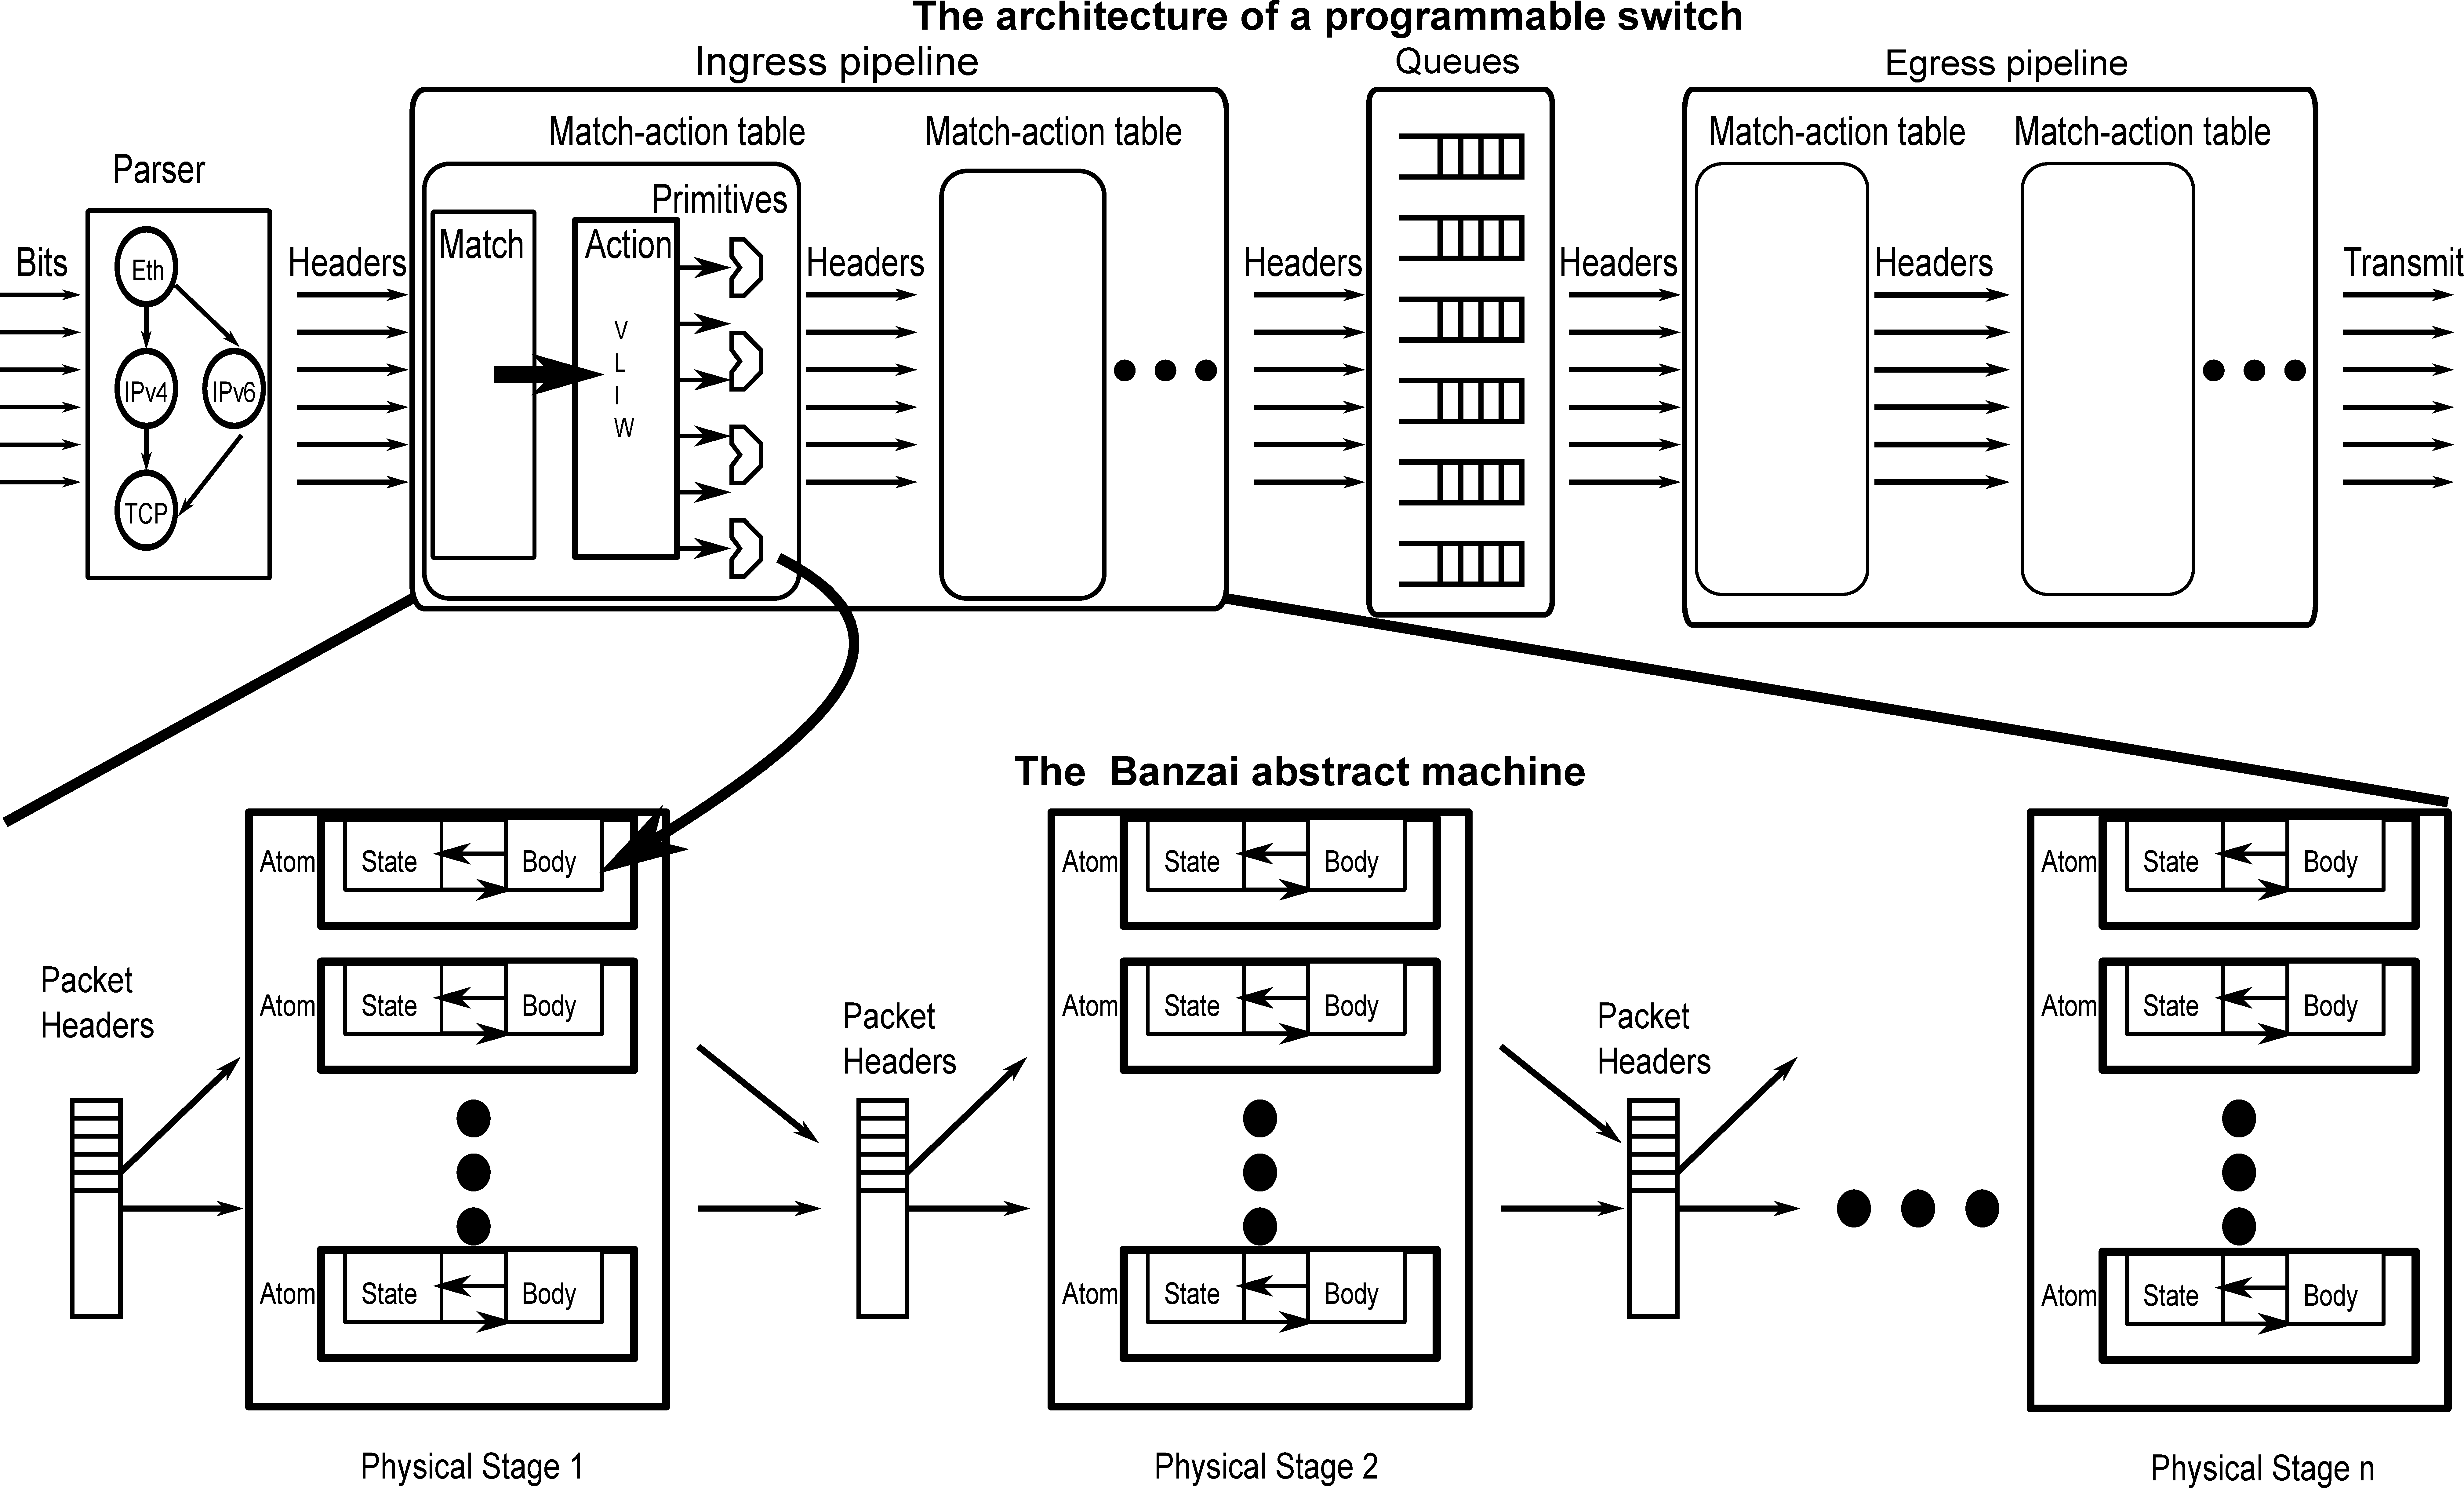
\includegraphics[width=\textwidth]{banzai.pdf}
  \caption{The \absmachine machine model and its relationship to
  programmable switch architectures.}
  \label{fig:switch}
\end{figure*}

\absmachine is a machine model for programmable line-rate switches that serves
as the compiler target for \pktlanguage programs.  \absmachine's design is
inspired by recent programmable switch architectures such as Barefoot's
Tofino~\cite{tofino}, Intel's FlexPipe~\cite{flexpipe}, and Cavium's XPliant
Packet Architecture~\cite{xpliant}. \absmachine abstracts these architectures
and extends them with stateful processing units to implement data-plane
algorithms. These processing units, called {\em atoms}, model the set of
operations that a hardware target can execute at line rate.

\subsection{Background: Programmable switches}
Packets arriving at a programmable switch~(Figure~\ref{fig:switch}) are parsed
by a programmable parser that turns packets into header fields. These header
fields are first processed by an ingress pipeline consisting of match-action
tables arranged in stages. Processing a packet at a stage may modify its header
fields as well as some persistent state at that stage. Each stage has access
only to its own local state. To share state between stages, it must be carried
forward in packet headers. Following the ingress pipeline, the packet is
queued. Once the packet is dequeued by the switch scheduler, it is processed by
a similar egress pipeline before being transmitted.

To reduce chip area, the ingress and egress pipelines are shared across switch
ports.  Each pipeline handles aggregate traffic belonging to all ports on the
switch, at all packet sizes.  For instance, a 64-port switch with a line rate
of 10 Gbits/s per port and a minimum packet size of 64 bytes needs to process
around a billion packets per second~\cite{rmt}.  Equivalently, with a clock
frequency of 1 GHz, each pipeline stage needs to process one packet every clock
cycle (1 ns).  The need to handle one packet per clock cycle is typical because
switches are designed for the highest port count and line rate for a given chip
area. We assume one packet per clock cycle throughout the paper.\footnote{For
concreteness, we assume a 1 GHz clock frequency.}
%TODO: Define line rate.

Having to process a packet every clock cycle in each stage greatly
constrains the operations that can be performed on each packet. In
particular, any packet operation that modifies state visible to the
next packet {\em must} finish execution in a single clock cycle (see
\S\ref{ss:atoms} for details). Because of this restriction,
programmable switching chips provide a small set of processing units
or primitives for manipulating packets and state in a stage, unlike in
software routers. These processing units determine what algorithms can
run on the switch at line rate.

The challenge for us is to develop primitives that allow a broad range of
data-plane algorithms to be implemented, and to build a compiler to map a
user-friendly description of an algorithm to the primitives provided by a
switch.

\subsection{The \absmachine machine model}

\absmachine (the bottom half of Figure~\ref{fig:switch}) models the data-plane
components of an ingress or egress switch pipeline, consisting of a number of
stages executing synchronously on every clock cycle. Each stage processes one
packet every clock cycle (1 ns) and hands it off to the next. \absmachine
models the computation within a match-action table in a stage (i.e., the action
half of the match-action table), but not the match semantics (e.g., direct, or
ternary) (we discuss how to embed these computations in a standard match-action
pipeline in \S\ref{ss:guards}).  \absmachine does not model packet parsing and
assumes that packets arriving to it are already parsed.

\subsection{Atoms: \absmachine's processing units}
\label{ss:atoms}

Each pipeline stage in \absmachine contains a {\em vector of
  atoms}. All atoms in the vector execute in parallel on every clock
cycle.  Informally, an atom is an atomic unit of packet processing
supported natively by a \absmachine machine.
The atoms provided by 
a \absmachine machine form its instruction set.
Atoms may modify persistent state stored on the
switch. In contrast to instruction sets for CPUs, GPUs, DSPs, and
NPUs, the atoms for a \absmachine machine need to be substantially
richer to run real-world data-plane algorithms at line rate. We
explain why with an example.

Suppose we need to atomically increment a state variable stored on the switch
to count packets. One approach would be to have hardware support for three
simple single-cycle operations: \textit{read} some memory in the first clock
cycle, \textit{add} one in the next, and \textit{write} it to memory in the
third. This approach, however, does not provide atomic isolation. To see why,
suppose packet $A$ increments the counter from 0 to 1 by executing the read,
add, and write operations at clock cycles 1, 2, and 3 respectively.  If packet
$B$ issues the read at time 2, it will increment the counter again from 0 to 1,
when it should be 2. Locks over the shared counter are a potential
solution. However, locking causes packet $B$ to wait during packet $A$'s
increment, and the switch no longer sustains line rate of one packet every
clock cycle.\footnote{Wait-free objects~\cite{herlihy_wait} are an alternative
  to locking, but are typically too complex for hardware.} CPUs employ microarchitectural
  techniques such as operand forwarding to address this problem, but these techniques
  suffer from occasional pipeline stalls, which prevents line-rate
  performance from being achieved.
%% TODO: Not mentioning that shared memory is costly. Because, while that's true.
%% there are parts of the switch pipeline that use it (such as the scheduler).

\absmachine provides an atomic increment operation in hardware with an {\em
atom} to read memory, increment it, and write it back in a single stage within
one clock cycle. It uses the same approach to implement other atomic operations
at line rate.

Formally, an atom is a body of sequential code. It may also contain internal
state local to the atom. An atom completes execution of the entire body of
sequential code, modifying a packet and any internal state before processing
the next packet. The designer of a programmable switch would develop these
atoms, and expose them to a switch compiler as the programmable switch's
instruction set.
%%\ac{does this mean we could have invented a new
%%instruction to represent each atom, and the current representation as a
%%body of (C-like?) sequential code is simply convenience for people to 
%%implement different banzai machines?}
%%No. You need someway to represent an atom's functionality to the compiler.
%% like expression trees / tiles for instruction selection.

Using this representation, a switch counter that wraps around at a
value of 100 can be written as the atom:\footnote{We use {\tt p.x} to
  represent field {\tt x} within a packet {\tt p} and {\tt x} to
  represent a state variable {\tt x} that persists across packets.}
\begin{lstlisting}[style=customc, numbers=none, frame=none]
if (counter < 99)
  counter++;
else
  counter = 0;
\end{lstlisting}
Similarly, a stateless operation like setting a packet field
(e.g. P4's {\tt modify\_field} primitive~\cite{p4spec}) can be written
as the atom:
\begin{lstlisting}[style=customc, numbers=none, frame=none]
  p.field = value;
\end{lstlisting}
Table~\ref{tab:templates} provides more examples of atoms.

We note that---unlike stateful atomic operations such as a counter---stateless
atomic operations are easier to support with basic packet-field arithmetic.
Consider, for instance, the operation {\tt pkt.f1 = pkt.f2 + pkt.f3 - pkt.f4}.
This operation does not modify any persistent switch state because it only
reads and writes packet fields. It can be implemented without violating
atomicity by using two atoms: one atom to add fields f2 and f3 in one pipeline
stage (clock cycle), and another to subtract f4 from the result in the next,
without having to provide one large atom that supports the entire operation.

%%\ac{but I thought you are still implement the whole thing as one single atom
%%right? What's the point here}
%% The point is we can implement this as two atoms without violating atomicity.
%% Explained above.

\subsection{Constraining atoms}
\label{s:atomConstraints}

\textbf{Computational limits:} Atoms need to execute atomically from one packet
to the next, implying that any state internal to the atom must be updated
before the next packet arrives. Further, packets may be separated by as little
as one clock cycle. To guarantee atomicity in the worst case, we mandate that
atom bodies finish execution within one clock cycle, and constrain atom bodies
to do so.

We constrain atom bodies by defining {\it atom templates}
(\S\ref{ss:code_gen}).  An atom template is a program that terminates within a
clock cycle and specifies exactly how the atom is executed. One example is an
ALU with a restricted set of primitive operations to choose from
(Figure~\ref{fig:alu_diag}). Atom templates allow us to create and experiment
with \absmachine machines with different atoms. As programmable switches
evolve, we expect that atoms will evolve as well, but constrained by the
clock-cycle requirement~(\S\ref{ss:perfprog}).
%TODO: Consider removing this last sentence or replacing it with how
%transistor scaling could improve how much we pack into these atoms.

\begin{figure}[h]
  \begin{subfigure}{0.4\columnwidth}
  \begin{center}
  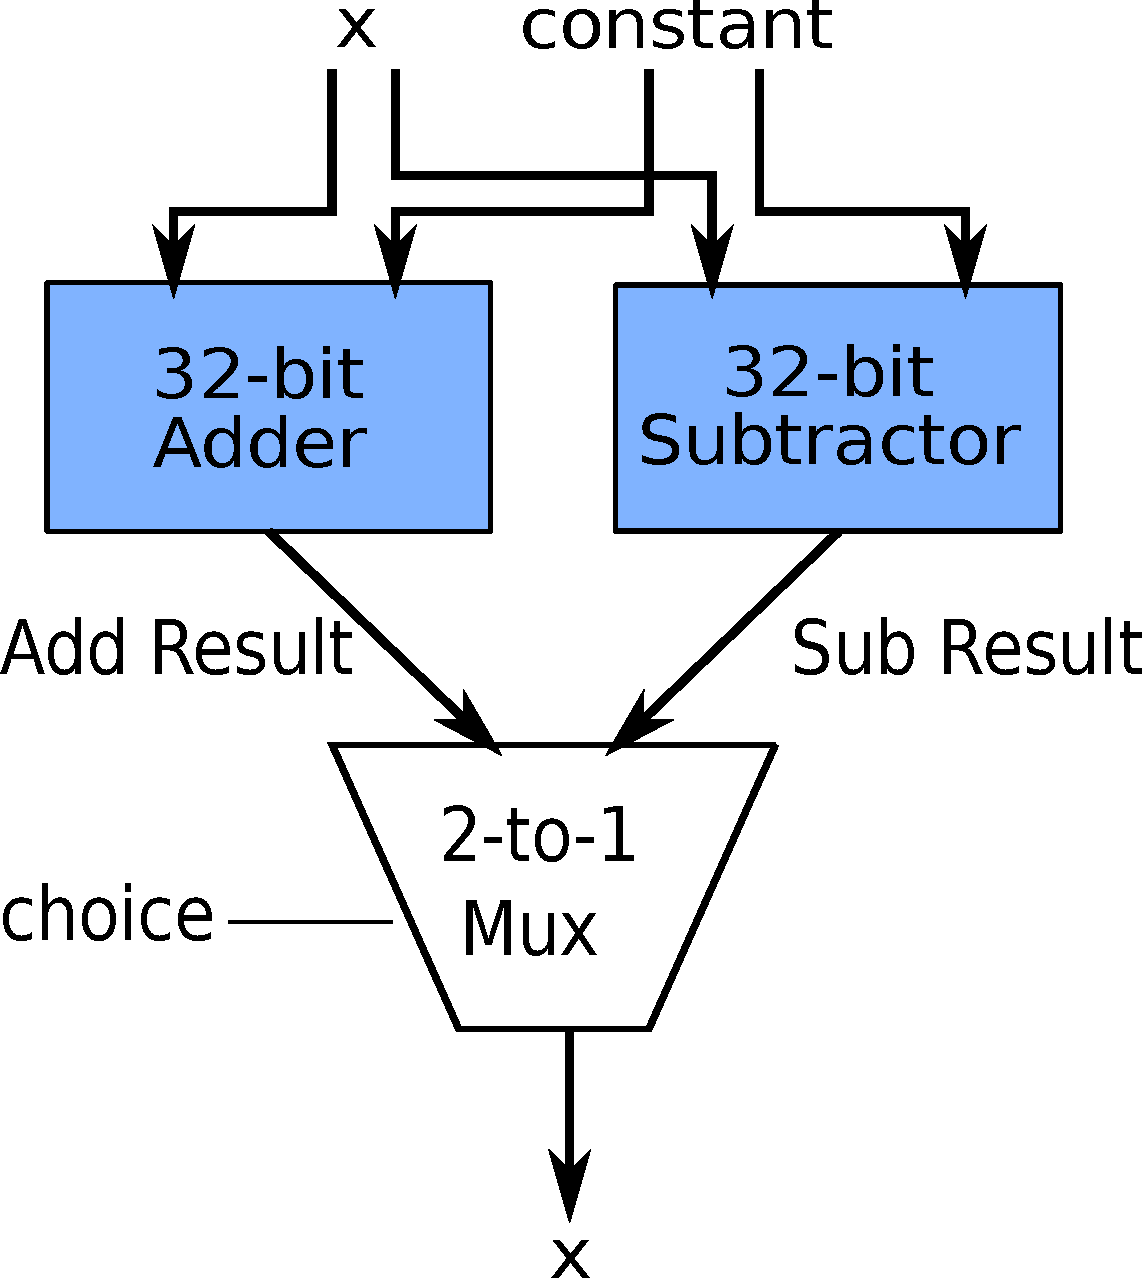
\includegraphics[width=\columnwidth]{circuit.pdf}
  \end{center}
  \caption{Circuit for an atom that can add or subtract a constant from a state variable.}
  \label{fig:alu_diag}
  \end{subfigure}
  \hspace{0.05\columnwidth}
  \begin{subfigure}{0.55\columnwidth}
  \begin{lstlisting}
  bit choice = ??;
  int constant = ??;
  if (choice) {
    x = x + constant;
  } else {
    x = x - constant;
  }
  \end{lstlisting}
  \caption{Circuit representation as an atom template.}
  %Each ``??(n)'' represents a hole that can be filled in with values in $[0, 2^n -1]$.}
  \label{fig:alu_in_sketch}
  \end{subfigure}
  \caption{Atoms and atom templates}
  \label{fig:atom}
\end{figure}

\textbf{Resource limits:} For any real machine, we also need to limit the
number of atoms in each stage (\textit{pipeline width}) and the number of
stages in the pipeline (\textit{pipeline depth}). This is similar to limits on
the number of stages, number of tables per stage, and amount of memory per
stage in programmable switch architectures such as RMT and
FlexPipe~\cite{lavanya_compiler}.

\subsection{What can \absmachine not do?}
\label{ss:limitations}

\absmachine is a good fit for data-plane algorithms that modify a small set of
packet headers and carry out small amounts of stateful or stateless computation
per packet. Data-plane algorithms like deep packet inspection and WAN
optimization require a switch to parse and process the packet payload as
well---effectively parsing a large ``header'' consisting of each byte in the
payload, which is challenging at line rates of 1 GHz. Such algorithms are best
left to general-purpose CPU platforms~\cite{e2}.  Some algorithms require
complex computations, but not on every packet.  For example, consider a
measurement algorithm that periodically scans a large table to perform garbage
collection.  \absmachine's atoms model small computations that occur on every
packet, and are not suitable for operations that span many clock cycles.

\section{Packet transactions}
\label{s:transactions}

\begin{figure*}[!t]
\begin{minipage}{0.5\textwidth}
\begin{small}
\begin{lstlisting}[style=customc]
#define NUM_FLOWLETS    8000
#define THRESHOLD       5
#define NUM_HOPS        10

struct Packet {
  int sport;
  int dport;
  int new_hop;
  int arrival;
  int next_hop;
  int id; // array index
};

int last_time [NUM_FLOWLETS] = {0};
int saved_hop [NUM_FLOWLETS] = {0};

void flowlet(struct Packet pkt) {
  pkt.new_hop = hash3(pkt.sport,
                      pkt.dport,
                      pkt.arrival)
                % NUM_HOPS;

  pkt.id  = hash2(pkt.sport,
                  pkt.dport)
            % NUM_FLOWLETS;

  if (pkt.arrival - last_time[pkt.id] @\label{line:ifStart}@
      > THRESHOLD)
  { saved_hop[pkt.id] = pkt.new_hop; } @\label{line:ifEnd}@

  last_time[pkt.id] = pkt.arrival;
  pkt.next_hop = saved_hop[pkt.id];
}
\end{lstlisting}
\end{small}
\caption{Flowlet switching written in \pktlanguage}
\label{fig:flowlet_code}
\end{minipage}
%
\vrule\quad
%
\begin{minipage}{0.4\textwidth}
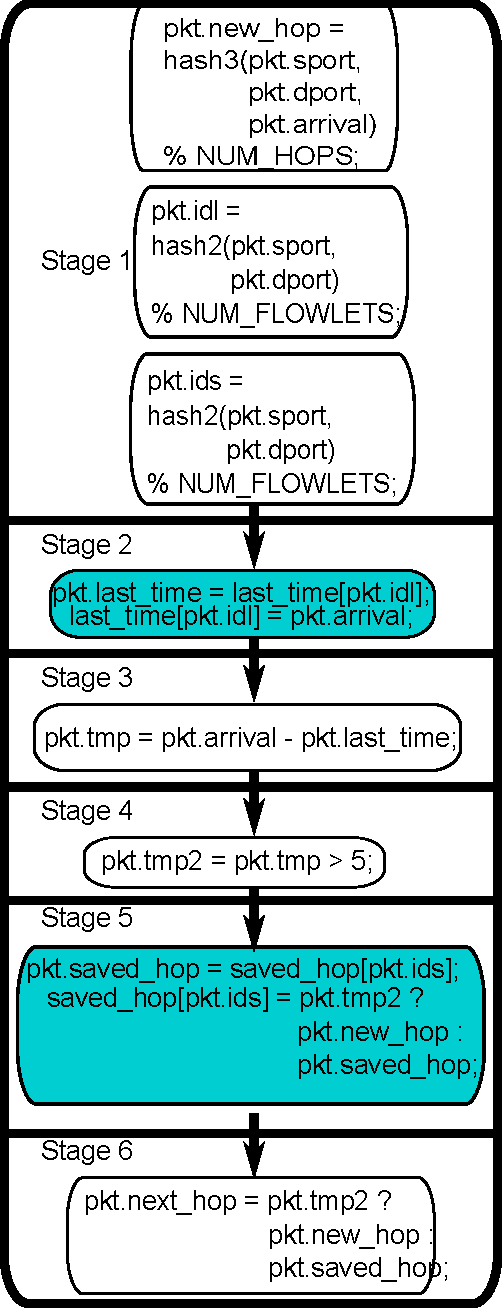
\includegraphics[width=0.8\columnwidth]{pipe.pdf}
\caption{Compiled 6-stage \absmachine pipeline implementing flowlet
switching.  Control flows from top to bottom. Atoms manipulating state are
shaded in blue.}
\label{fig:flowlet_pipeline}
\end{minipage}
\end{figure*}

To program a data-plane algorithm, a programmer would write code in
\pktlanguage using packet transactions (Figure~\ref{flowlet_code}) and then use
the \pktlanguage compiler to compile to an atom pipeline for a \absmachine
machine (Figure~\ref{fig:flowlet_pipeline}). We first describe packet
transactions in greater detail by walking through an example
(\S\ref{ss:flowlet}). Next, we discuss constraints in \pktlanguage
(\S\ref{ss:constraints}) informed by the domain of line-rate switches. We then
discuss how packet transactions are triggered (\S\ref{ss:guards}) and how
multiple transactions are handled (\S\ref{ss:multiple}).

\subsection{\pktlanguage by example}
\label{ss:flowlet}

We now illustrate programming using packet transactions in \pktlanguage, using
flowlet switching~\cite{flowlets} as an example. Flowlet switching is a
load-balancing algorithm that sends bursts of packets (called flowlets) from a
TCP flow on different paths, provided the bursts are separated by a large
enough time interval to ensure packets do not arrive out of order at a TCP
receiver. Figure~\ref{fig:flowlet_code} shows flowlet switching in
\pktlanguage. For simplicity, we hash only the source and destination ports; it
is easy to extend it to the full 5-tuple.

This example demonstrates the core language constructs in \pktlanguage. All
packet processing happens in the context of a packet transaction (the function
\texttt{flowlet} starting at line 17). The function's argument {\tt pkt}
declares the fields in a packet (lines 5--12)\footnote{We use fields to refer
to both packet headers such as source port ({\tt sport}) and destination port
({\tt dport}) and packet metadata ({\tt id}).} that can be referenced by the
function body (lines 18--32).  The function body can also modify persistent
switch state using global variables (e.g.  \texttt{last\_time} and
\texttt{saved\_hop} on lines 14 and 15, respectively).

Conceptually, the switch invokes the packet transaction function on each
incoming packet sequentially. To the programmer, the function modifies the
passed-in packet argument and runs to completion before processing the next
packet.  The function may invoke \textit{intrinsics} such as \texttt{hash2} on
line 23 to use hardware accelerators such as hash generators.  The \pktlanguage
compiler uses an intrinsic's signature to infer dependencies and supplies a
canned run-time implementation, but otherwise does not analyze an intrinsics's
internal behavior. When compiled to a \absmachine machine
(\S\ref{s:absmachine}), the \pktlanguage compiler (\S\ref{s:compiler}) converts
the code in Figure~\ref{fig:flowlet_code} into the atom pipeline in
Figure~\ref{fig:flowlet_pipeline}.

\subsection{Constraints on the language}
\label{ss:constraints}

The overall language is a constrained subset of C
(Table~\ref{tab:restrict}).  These constraints are required for
deterministic performance.  Memory allocation, unbounded iteration
counts, and unstructured control flow all cause variable performance,
which may prevent an algorithm from achieving line rate.
Furthermore, all accesses to a given array within one execution of a
transaction, i.e. one packet, must use the same array index. For
example, all read and write accesses to the array \texttt{last\_time}
use the index \texttt{pkt.id}, which is constant for each packet, but
can change between packets. This restriction mirrors restrictions on
memories, where supporting distinct read and write addresses every
clock cycle is challenging.
%TODO: Try and address this.
%\MA{Do we model this restriction in PISA?
%  It would be better to add it to Sec 2.}

\begin{table}
  \begin{tabular}{p{0.9\columnwidth}}
    No iteration (while, for, do-while).\\
    No goto, break, or continue.\\
    No pointers.\\
    No dynamic memory allocation / heap.\\
    Array index is constant for each transaction execution.\\
    No access to data i.e. unparsed portion of the packet.\\
    No arrays in packet fields.\\
  \end{tabular}
  \caption{Restrictions in \pktlanguage}
  \label{tab:restrict}
\end{table}

\subsection{Triggering packet transactions}
\label{ss:guards}
Packet transactions specify \textit{how} to process packet headers and/or
state.  To specify {\em when} to run packet transactions, we provide a {\em
guard}: a predicate on packet fields that triggers the transaction whenever a
packet matches the guard. An example guard would execute heavy-hitter detection
on all packets arriving on a specific port. The guard can be implemented using
the match key in a match-action pipeline, with the actions being the atoms
resulting from compiling packet transactions to a pipeline of atoms. Because
guards can be easily integrated into a standard match-action pipeline, this
paper only focuses on packet transactions.

\subsection{Handling multiple transactions}
\label{ss:multiple}
So far, we have discussed a single packet transaction. In practice, a switch
would run multiple data-plane algorithms each processing its own subset of
packets. To accommodate multiple transactions, we envision providing a policy
language that specifies pairs of guards and transactions. Realizing a policy is
straightforward when all guards are disjoint. When guards overlap, mutliple
transactions may need to execute on the same subset of packets, requiring a
mechanism to compose two transactions. One approach is to concatenate the two
transaction bodies in an order specified by the user, providing the illusion of
a larger transaction that combines two transactions. We leave a detailed
exploration of these approaches to future work. For the rest of this paper, we
focus only on compiling a single packet transaction.

\section{The \pktlanguage compiler}
\label{s:compiler}

\begin{figure*}[!t]
  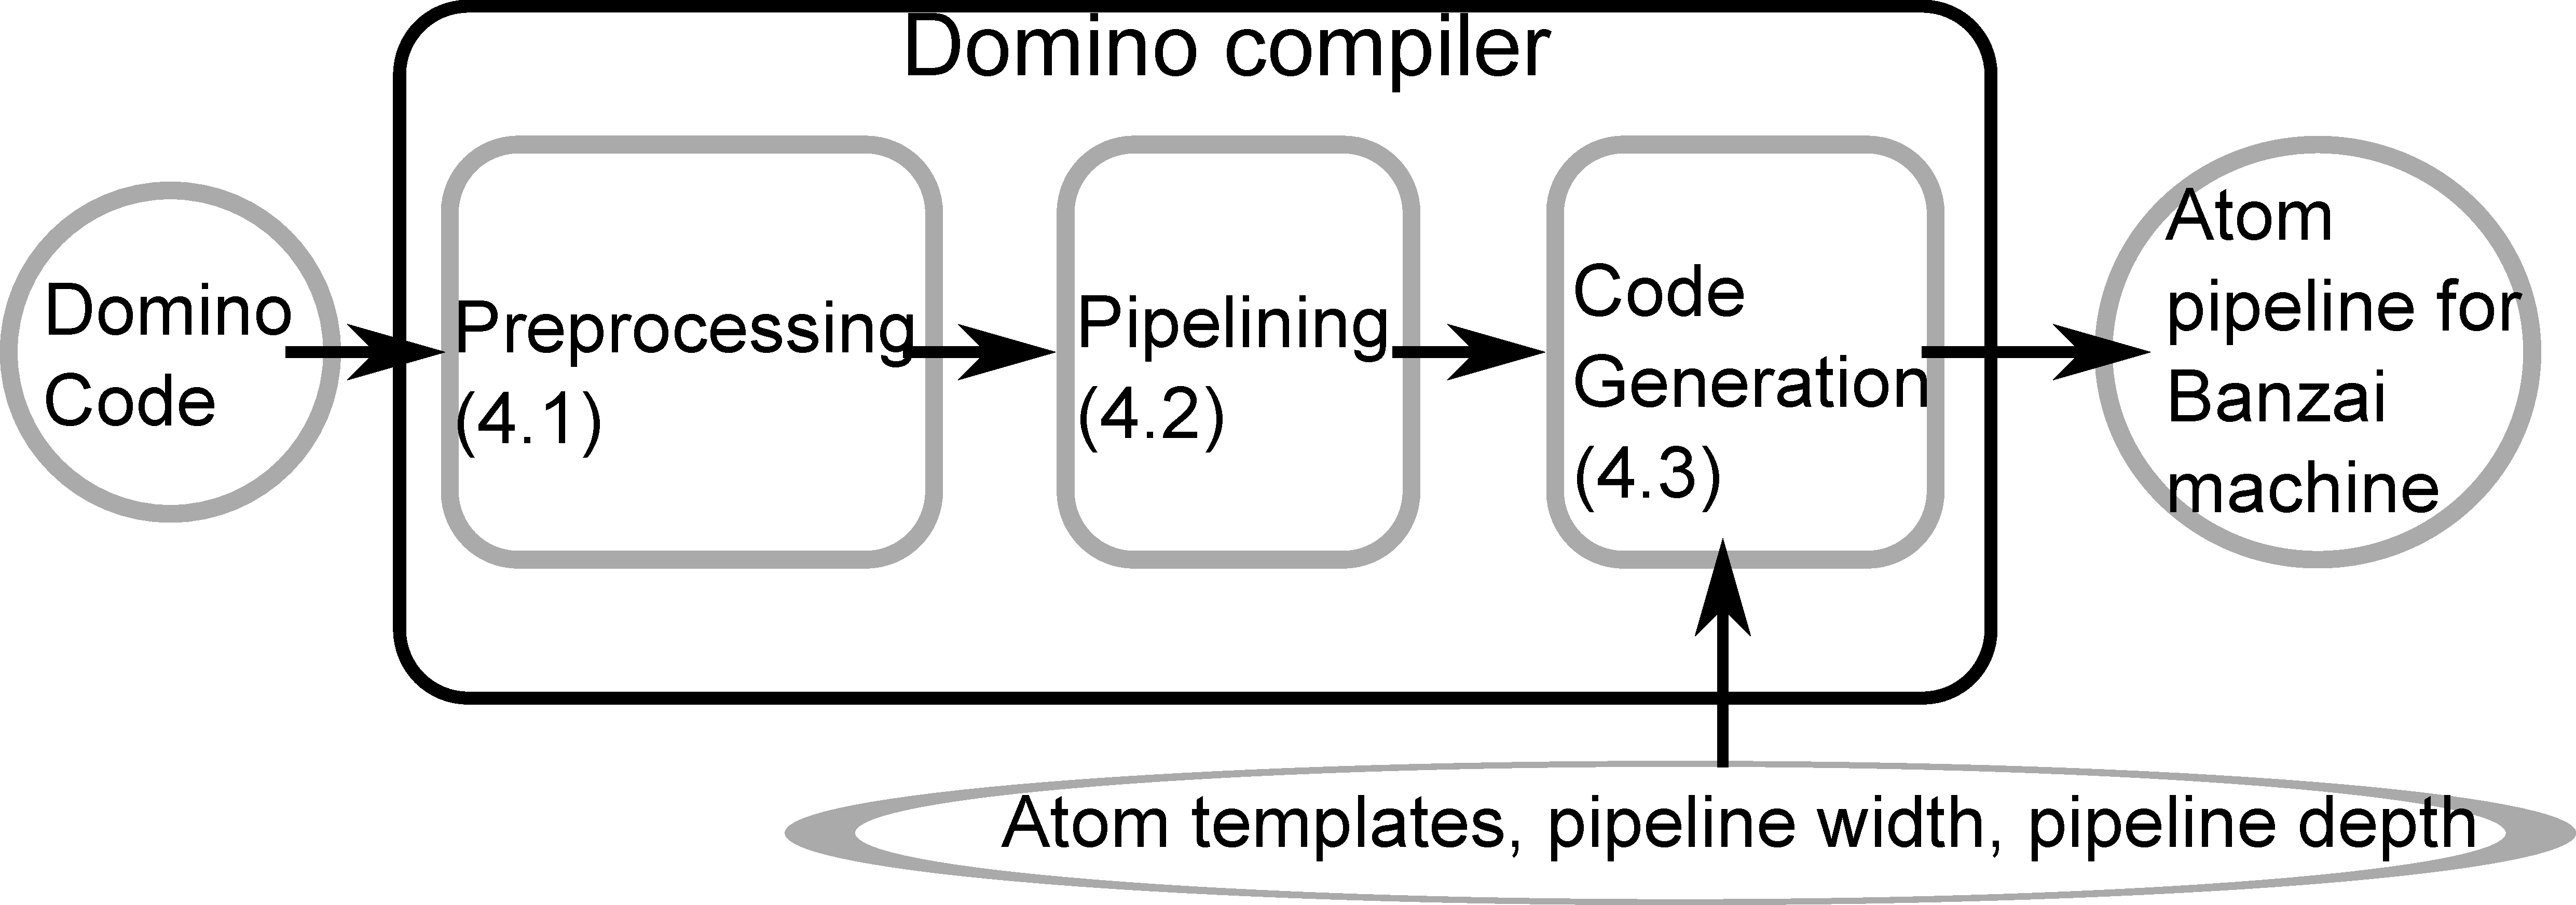
\includegraphics[width=\textwidth]{compiler.pdf}
  \caption{Passes in the \pktlanguage compiler}
\end{figure*}

The \pktlanguage compiler borrows several well-established techniques from the
compiler literature~\cite{muchnik}. However, as we show throughout this
section, constraining \pktlanguage for deterministic performance has a happy
side effect: it allows us to considerably simplify the \pktlanguage compiler
relative to mainstream compilers.

\subsection{Lexing, parsing, and semantic analysis}
Because \pktlanguage's syntax is based on C, we use clang's library
interface~\cite{libclang} to generate an Abstract Syntax Tree (AST) for packet
transactions written in \pktlanguage. The remaining compiler passes operate on
this AST. Basing \pktlanguage's syntax on C has several benefits.  Clang's
frontend catches several errors with no additional effort. It also
allows us to use the C macro preprocessor for constants. Intrinsic
functions representing hardware primitives (e.g.  hashes), can be
implemented using arbitrary C code and linked with \pktlanguage code before
running the resulting binary on a \absmachine machine.
%(\S\ref{ss:verification}).

\subsection{If-conversion to straight-line code}
A packet transaction's body can contain if-else statements that alter control
flow and complicate dependence analysis. We eliminate if-else statements by
transforming them into the C conditional operator, starting from the innermost
if statements and recursing outwards (Figure~\ref{fig:if_convert}). This
procedure is called if-conversion~\cite{if_conversion}; it is much simpler in
\pktlanguage because only if-else statements alter control flow in
\pktlanguage; all other control transfer (break, continue, loops) is forbidden.
This transformation creates straight-line code, where control passes
sequentially without branching. Straight-line code simplifies the rest of the
compiler, like computing the SSA(\S\ref{ss:ssa}).

\begin{figure*}[!t]
  \begin{minipage}{0.47\textwidth}
  \begin{small}
  \begin{lstlisting}[style=customc]
if (pkt.arrival -
    last_time[pkt.id] >
    THRESHOLD) {
 saved_hop[pkt.id] = pkt.new_hop;
}
  \end{lstlisting}
  \end{small}
  \end{minipage}
  \begin{minipage}{0.53\textwidth}
  \begin{small}
  \begin{lstlisting}[style=customc]
pkt.tmp = pkt.arrival -
          last_time[pkt.id]
          > THRESHOLD;
saved_hop[pkt.id] = pkt.tmp ?
                    pkt.new_hop :
                    saved_hop[pkt.id];
  \end{lstlisting}
  \end{small}
  \end{minipage}
\caption{Conversion to straight-line code}
\label{fig:if_convert}
\end{figure*}
\subsection{Converting state variables to load/store form}

We next identify state variables used in a packet transaction, both arrays and
scalars, such as \texttt{last\_time} and \texttt{saved\_hop} in
Figure~\ref{fig:flowlet}. For each state variable, we create a \textit{read
flank} to read the state variable into a temporary packet field. For an array,
we also move the index expression into the read flank, exploiting the fact that
only one array index is accessed by each packet in valid \pktlanguage
programs.  Then, we replace all occurrences of the state variable with the
packet temporary, and create a \textit{write flank} to write the packet
temporary back into the state variable.  Figure ~\ref{fig:stateful_flanks}
illustrates this transformation on a fragment.  After this pass, the code
resembles code for a load-store architecture~\cite{load_store}: state variables
only support reads and writes; arithmetic happens on packet variables.
Restricting the operations on state variables simplifies their treatment
during code partitioning (\S\ref{ss:partitioning}).


\begin{figure*}[!t]
  \begin{minipage}{0.47\textwidth}
  \begin{small}
  \begin{lstlisting}[style=customc]
pkt.id = hash2(pkt.sport,
               pkt.dport)
         % NUM_FLOWLETS;
last_time[pkt.id] = pkt.arrival;
  \end{lstlisting}
  \end{small}
  \end{minipage}
  \begin{minipage}{0.53\textwidth}
  \begin{small}
  \begin{lstlisting}[style=customc]
// Read flank for last_time
pkt.id = hash2(pkt.sport,
                pkt.dport)
         % NUM_FLOWLETS;
pkt.last_time = last_time[pkt.id];

pkt.last_time = pkt.arrival;

// Write flank for last_time
last_time[pkt.id] = pkt.last_time;
  \end{lstlisting}
  \end{small}
  \end{minipage}
  \caption{Adding read and write flanks}
\label{fig:stateful_flanks}
\end{figure*}

\subsection{Renaming variables to static single-Assignment Form}
\label{ss:ssa}

We next convert to static single-assignment form (SSA)~\cite{ssa}, an
intermediate form used by many compilers~\cite{tree_ssa, llvm}.  In SSA, every
variable is assigned exactly once. To compute the SSA, we replace every
definition of a packet variable with a new packet variable and propagate this
new packet variable until the next definition of the same variable. State
variables are already in SSA form: after their flanks have been added, every
state variable is written exactly once in the write flank.  While general
algorithms for computing the SSA are fairly involved~\cite{ssa}, \pktlanguage's
SSA computation is simpler because it operates on straight-line code.  SSA
simplifies further analysis. Every variable is assigned exactly once, implying
that there are no Write-After-Read or Write-After-Write dependencies. Only
Read-After-Write dependencies remain, simplifying dependency
analysis during code partitioning (\S\ref{ss:partitioning}).

\begin{figure*}[!t]
  \begin{minipage}{0.48\textwidth}
  \begin{small}
  \begin{lstlisting}[style=customc]
pkt.id = hash2(pkt.sport,
               pkt.dport)
               % NUM_FLOWLETS;
pkt.last_time = last_time[pkt.id];
pkt.last_time = pkt.arrival;
last_time[pkt.id] = pkt.last_time;
  \end{lstlisting}
  \end{small}
  \end{minipage}
  \begin{minipage}{0.52\textwidth}
  \begin{small}
  \begin{lstlisting}[style=customc]
pkt.id0 = hash2(pkt.sport,
                pkt.dport)
                % NUM_FLOWLETS;
pkt.last_time0 = last_time[pkt.id0];
pkt.last_time1 = pkt.arrival;
last_time[pkt.id0] = pkt.last_time1;
  \end{lstlisting}
  \end{small}
  \end{minipage}
  \caption{SSA transformation}
\label{fig:ssa}
\end{figure*}

\begin{figure*}[!t]
\begin{lstlisting}[style=customc]
pkt.id            = hash2(pkt.sport, pkt.dport) % NUM_FLOWLETS;
pkt.saved_hop     = saved_hop[pkt.id]; @\label{line:stateRead}@
pkt.last_time     = last_time[pkt.id];
pkt.new_hop       = hash3(pkt.sport, pkt.dport, pkt.arrival) % NUM_HOPS;
pkt.tmp           = pkt.arrival - pkt.last_time;
pkt.tmp2          = pkt.tmp > THRESHOLD;
pkt.next_hop      = pkt.tmp2 ? pkt.new_hop : pkt.saved_hop;
saved_hop[pkt.id] = pkt.tmp2 ? pkt.new_hop : pkt.saved_hop; @\label{line:stateWrite}@
last_time[pkt.id] = pkt.arrival;
\end{lstlisting}
\caption{Flowlet switching in three-address code}
\label{fig:three_address}
\end{figure*}

\subsection{Expression flattening to three-address code}
We next transform into three-address code~\cite{tac}, where all instructions
are either reads / writes into stateful variables or carry out packet
manipulations of the form: \texttt{pkt.f1 = pkt.f2 op pkt.f3;} where
\texttt{op} includes all arithmetic, logical, and relational operators. We also
allow either pkt.f2 or pkt.f3 to be an intrinsic function call, because we
assume these are supported in hardware. To generate three-address code, we
flatten expressions that are not already legal in three-address code, by
introducing enough temporaries
(Figure~\ref{fig:three_address}).
%Three-address code instructions are similar to P4's action
%primitives~\cite{p4spec} and RMT's VLIW instruction set~\cite{rmt}. 

\subsection{Code partitioning to codelets}
\label{ss:partitioning}
At this point, the code is still sequential. Code partitioning turns sequential
code into a pipeline of \textit{codelets}, where each codelet is a small
sequential block of three-address code statements. We generate this pipeline of
codelets, by exploiting parallelism within and across pipeline stages.
Subsequently, we map each codelets one-to-one to atoms provided by a particular
\absmachine machine~(\S\ref{ss:code_gen}), returning a compiler error if any
codelet doesn't map to an atom provided by the hardware.

To partition code into codelets, we carry out the following steps:
\begin{CompactEnumerate}
  \item Create a node for each statement (Figure~\ref{fig:three_address}) in
    the packet transaction after expression flattening.
  \item Create a bidirectional edge between N1 and N2 where N1 is a read from a
    state scalar / state array and N2 is a write into the same state scalar /
    state array. This step captures the constraint that state is internal to an
    atom in \absmachine. Because state variables don't occur in any
    instructions besides reads and writes, this is all we need to do to handle
    state variables.
  \item Create an edge (N1, N2) for every pair of nodes N1, N2 where N2 reads
    a variable written by N1. We only check read-after-write dependencies because
    control dependencies turn into data dependencies when generating straight-line
    code. Further, the use of SSA removes all write-after-read and write-after-write
    dependencies.
  \item Generate strongly connected components (SCCs) of the resulting graph
    (Figure~\ref{fig:partitioning}a) and condense the SCCs to to create a directed
    acyclic graph (DAG) (Figure~\ref{fig:partitioning}b). This step captures the
    constraint that all operations on state variables (read, write, and modify)
    must reside within the same atom because state is local to an atom.
  \item Schedule the resulting DAG using critical path
    scheduling~\cite{crit_path_sched}, creating a new pipeline stage every time
    one operation needs to follow another (Figure~\ref{fig:flowlet}b).
\end{CompactEnumerate}
At this point, the resulting codelet pipeline (Figure~\ref{fig:flowlet}b)
implements the packet transaction.  Further, the codelets themselves have a
stylized form.  Codelets that don't manipulate state contain exactly one
three-address code instruction. Codelets that manipulate state contain at least
two statements: a read from a state variable and a write to a state variable
and optionally consist of one or more updates to the state variable through
packet temporaries.

\begin{figure*}[!t]
\begin{minipage}{0.5\textwidth}
  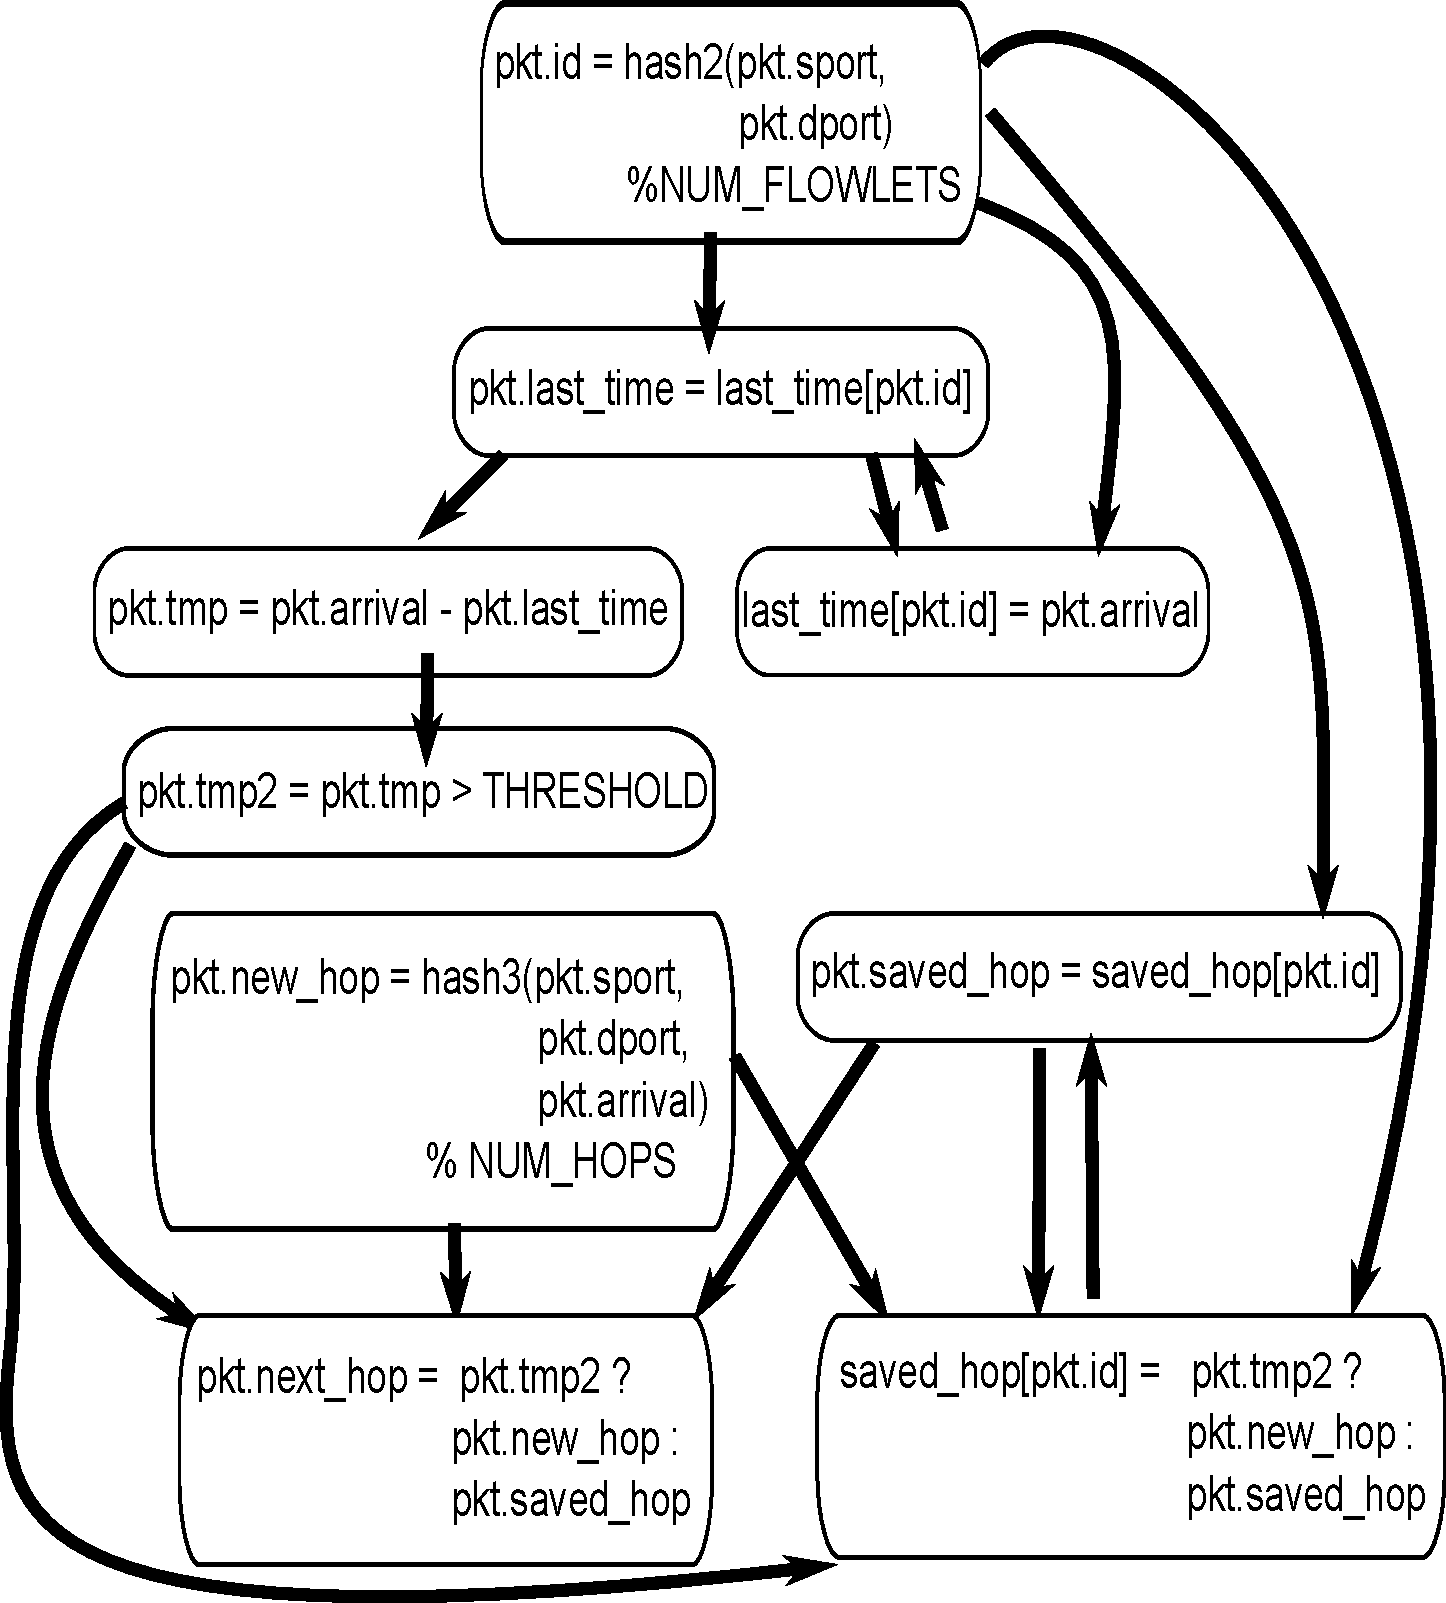
\includegraphics[width=\columnwidth]{deps.pdf}
\end{minipage}
%
\vrule\quad
%
\begin{minipage}{0.5\textwidth}
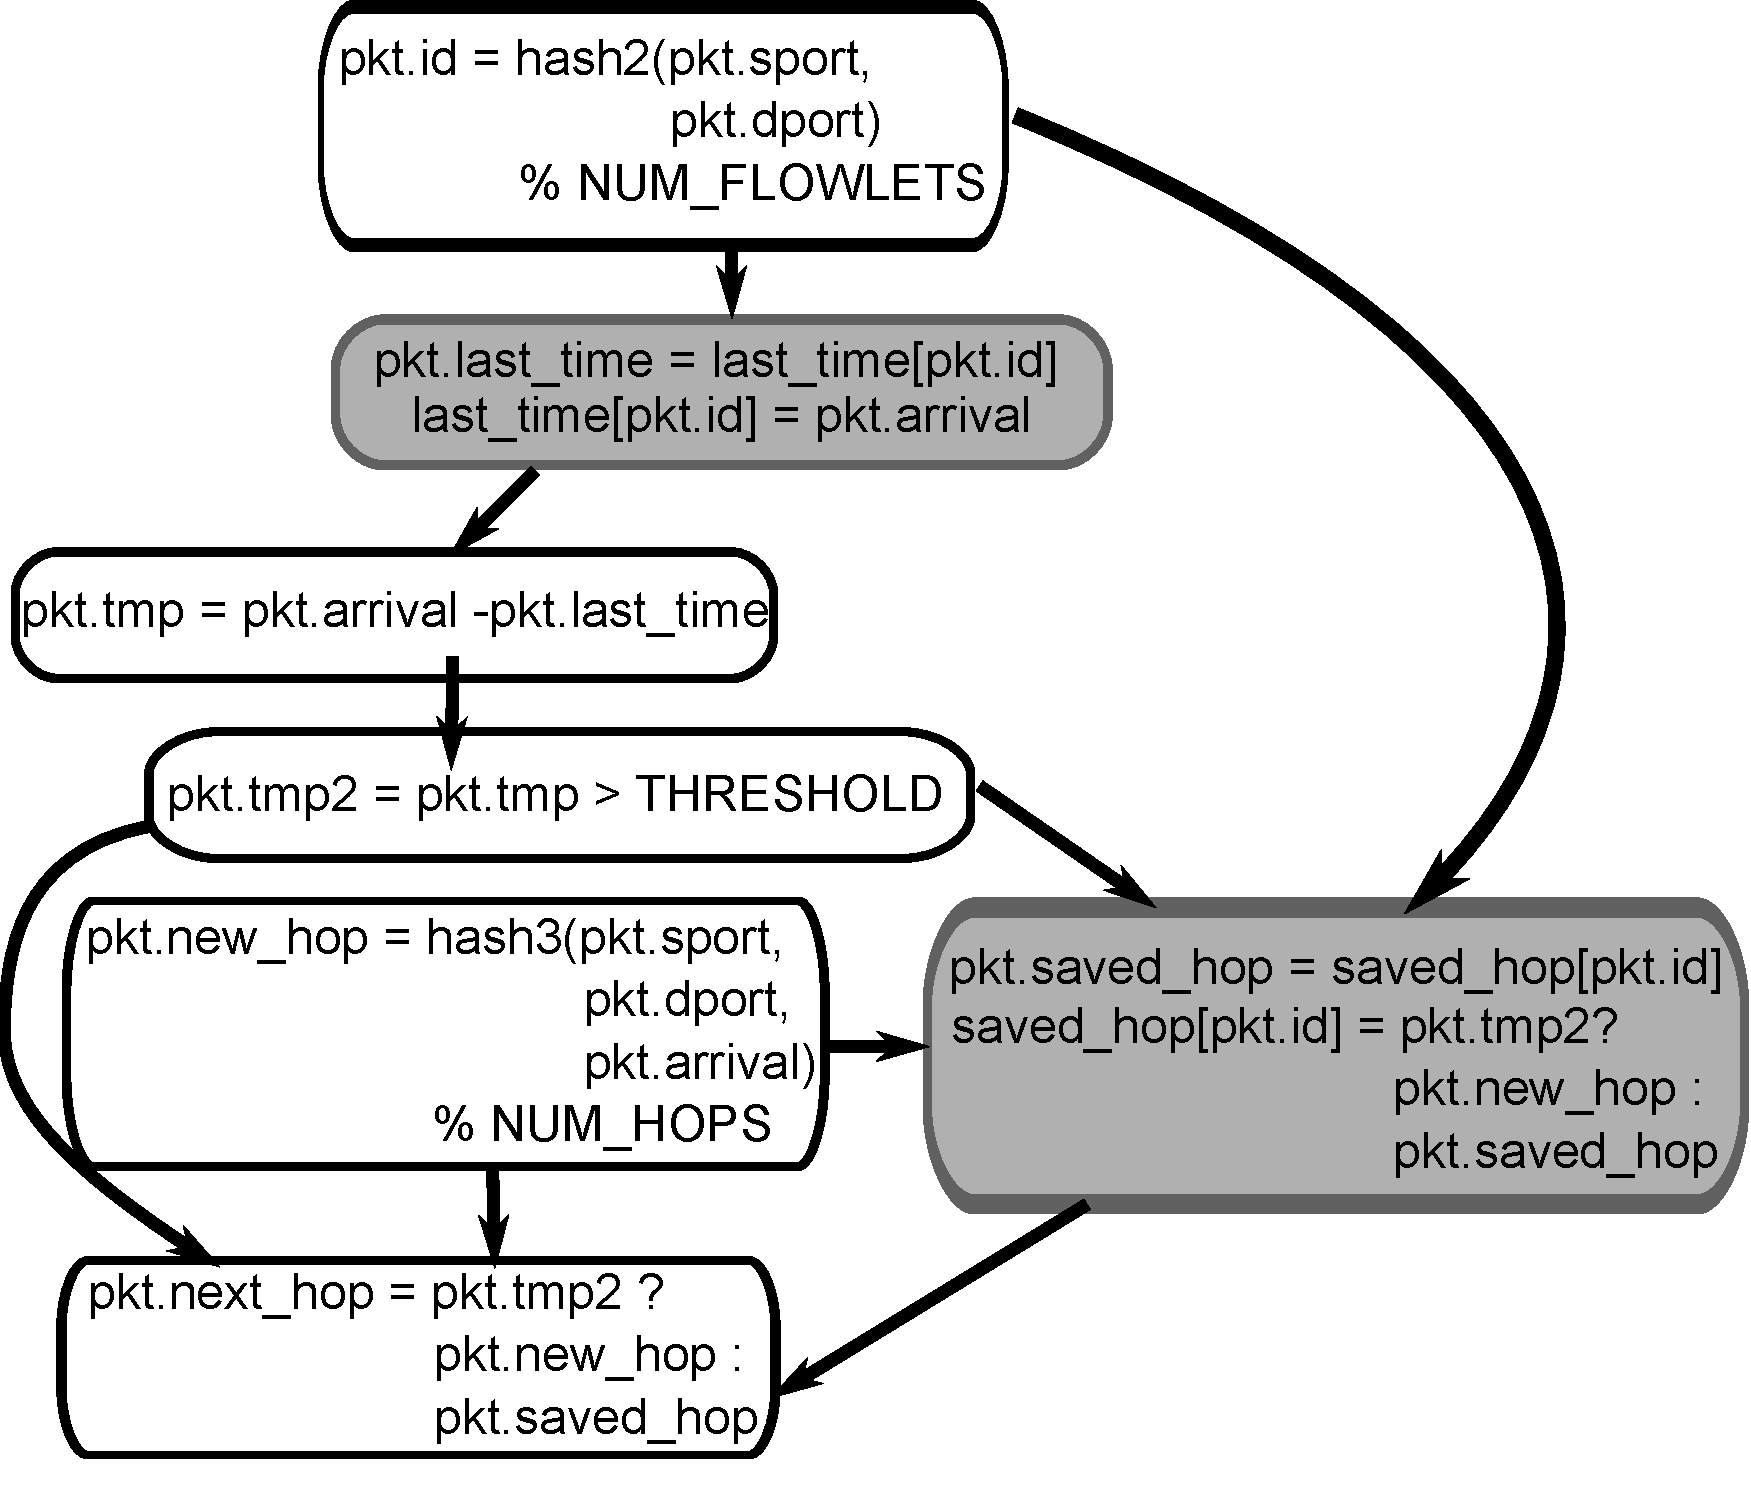
\includegraphics[width=\columnwidth]{scc.pdf}
\end{minipage}
\caption{Dependency graph (a) before and (b) after condensing strongly connected components}
\label{fig:partitioning}
\end{figure*}

\subsection{Code generation: Mapping a codelet to an atom}
\label{ss:code_gen}
Next, we determine how the codelets created by code partitioning in the
previous step map one-to-one to atoms provided by the \absmachine machine. We
consider codelets that do and don't manipulate state separately because we
handle each differently.

\textbf{Stateless codelets}
Expression flattening generates stateless codelets that each have only one
instruction in three-address code form (e.g. any of the unshaded boxes in
Figure~\ref{fig:flowlet}b). For this paper, we assume that all \absmachine
machines support all atoms that correspond to a single statement in
three-address code form. This assumption is backed by the fact that P4's
primitives~\cite{p4spec} and RMT's VLIW action set~\cite{rmt} both contain
instructions that are in three-address code form. With this assumption, mapping
a stateless codelet to an atom is trivial: each stateless codelet produced by
code partitioning has exactly one three-address code instruction, which is
equivalent to an atom available in the \absmachine machine. If the \absmachine
machine supports complex atoms beyond three-address code instructions, this
approach is still correct, although suboptimal. For instance, if the
\absmachine machine supports a multiply-and-accumulate atom~\cite{mac},
expression flattening would generate two atoms (one each for the multiply and
accumulate), where one suffices.

\textbf{Stateful codelets}
Stateful codelets have multi-line bodies that need to execute atomically. For
instance, updating the state variable \texttt{saved\_hop} in
Figure~\ref{fig:flowlet}b requires a read, followed by a conditional write.  It
is not readily apparent whether these codelets can be mapped to an available
atom. We develop a general technique to determine the implementability of such
stateful codelets, given as input the stateful atom template provided by the
\absmachine machine.

An atom template defines a space of possible computations (such as different
ALU operations, or different permitted sequences of $N$ three-address
instructions).  The exact computation is selected by \textit{configuring} the
atom. The codelet is a specification that is to be checked for functional
equivalence against one of the atom configurations supported by the atom
template. In other words, we need to \textit{synthesize} the atom's
\textit{configuration}, given an \textit{atom template} describing the atom's
functionality.

This is the realm of syntax-guided program synthesis~\cite{sgsyn}, where the
programmer supplies a partial program or template (hence the term
syntax-guided) with missing details, and a specification. A \textit{program synthesis
tool} then synthesizes these details in the partial program to ensure it matches
up bit exactly with the specification. One such program synthesis tool is
SKETCH~\cite{bitstreaming, sketch_asplos, sketch_manual}, which allows the
programmer to specify a partial program with \textit{holes} that are then
``filled in'' by SKETCH to match the specification
(Figure~\ref{fig:sketch}).

\begin{figure}[!b]
  \begin{center}
  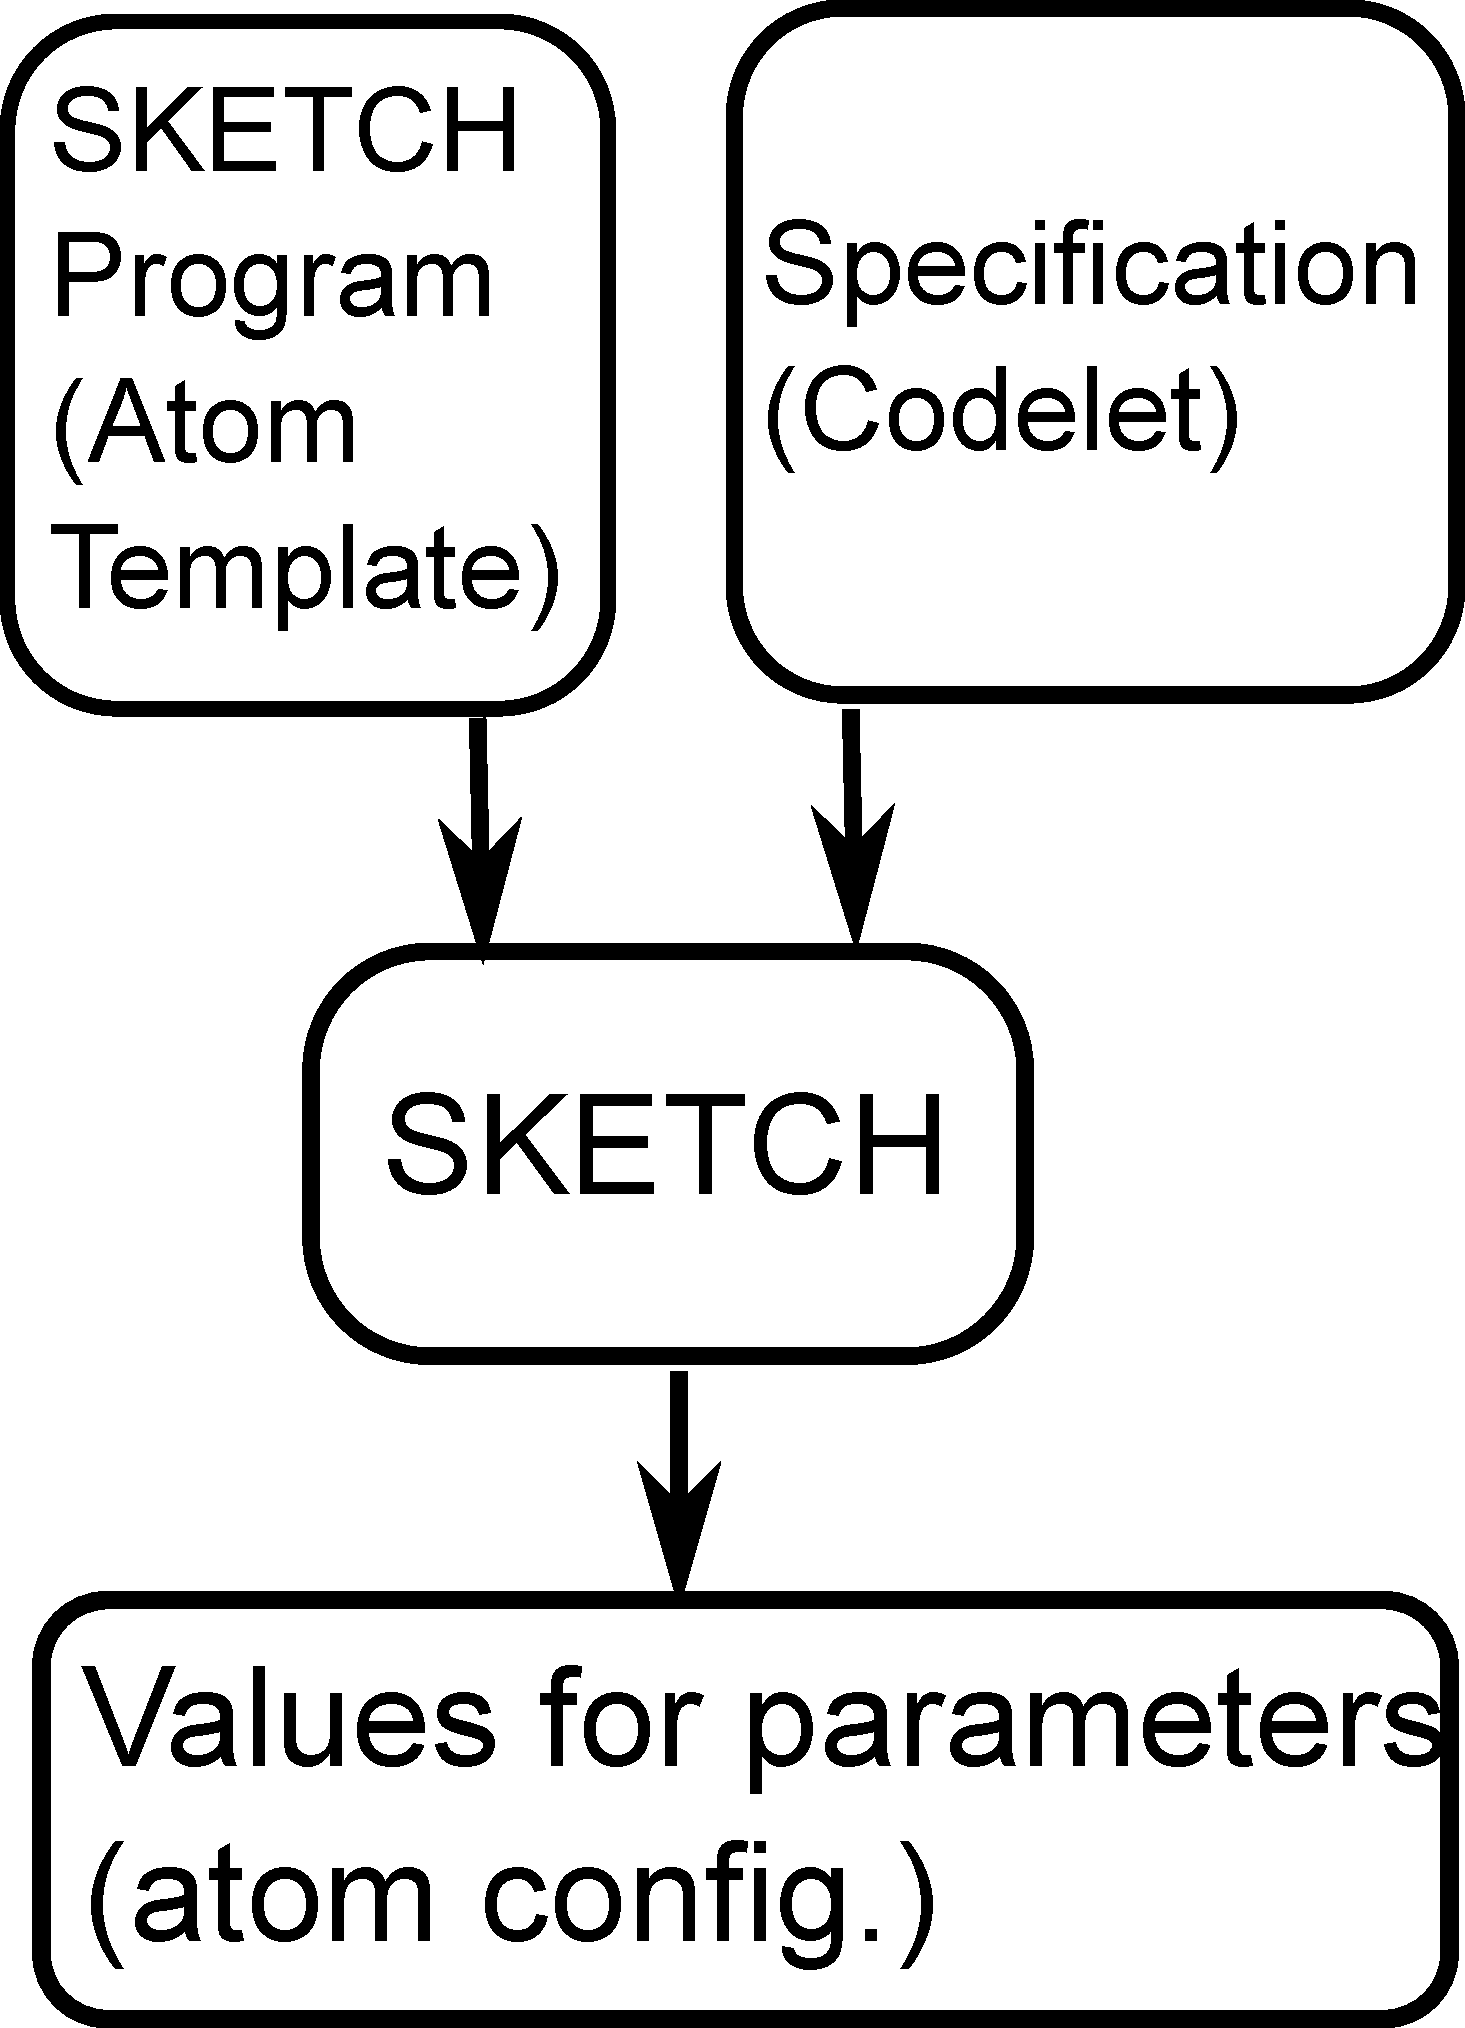
\includegraphics[width=0.4\columnwidth]{sketch.pdf}
  \caption{Overview of SKETCH and its application to atom configuration}
  \label{fig:sketch}
  \end{center}
\end{figure}

\begin{figure}[h]
  \begin{minipage}{0.4\columnwidth}
  \begin{center}
  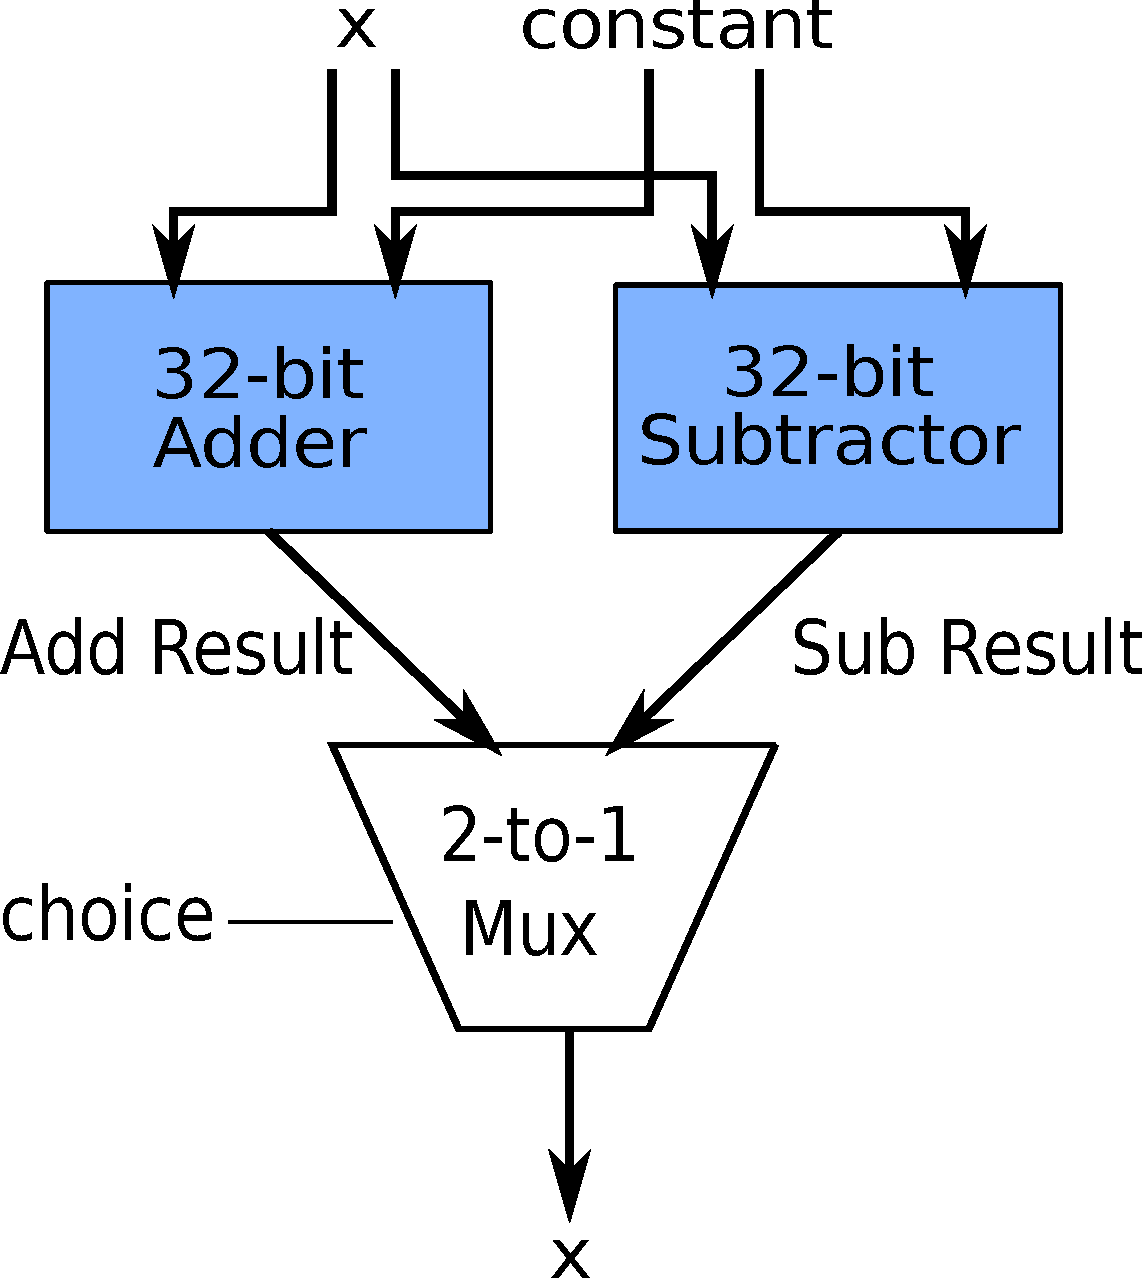
\includegraphics[width=\columnwidth]{circuit.pdf}
  \end{center}
  \end{minipage}
  \begin{minipage}{0.55\columnwidth}
  \begin{center}
  \begin{lstlisting}
  bit choice = ??(1);
  int constant = ??(16);
  if (bit) {
    x = x + constant;
  } else {
    x = x - constant;
  }
  \end{lstlisting}
  \end{center}
  \end{minipage}
\caption{\small (a) Circuit for an atom that can either add or subtract a
constant from a state variable.  (b) Circuit's representation in SKETCH.
Each ``??(n)'' represents a hole that can be filled in with values in
  $[0, 2^n -1]$.}
\label{fig:alu_in_sketch}
\end{figure}

We use SKETCH to solve the atom configuration problem.  Consider an atom
template that models an ALU (Figure~\ref{fig:alu_in_sketch}a) taking two
configuration parameters: an opcode, \texttt{choice}, specifying an addition or subtraction
operation, and a 16-bit positive constant, \texttt{constant}.  The ALU's functionality is to add
or subtract this constant from one state variable. This ALU can be represented
by the SKETCH partial program given in Figure~\ref{fig:alu_in_sketch}b.

Let's say we want to map the codelet x=x+1 to this atom. The codelet is then
fed into SKETCH as the desired specification and the atom template is fed into
SKETCH as the partial program (Figure~\ref{fig:sketch}). SKETCH will configure
the atom template by setting \texttt{choice} to 0 and \texttt{constant} to 1.
On the other hand, if the codelet x = x * x was supplied as the specification,
SKETCH will return an error because the specification cannot be mapped to any
of the computations provided by the atom template. We don't describe the
algorithms underlying SKETCH because we treat SKETCH as a blackbox in the
\pktlanguage compiler. The interested reader is referred to~\cite{bitstreaming,
sketch_asplos} for a more detailed treatment of these topics.

Using SKETCH to represent atom templates allows us to express the behavior of
diverse atoms (Table~\ref{tab:templates}) using a natural imperative syntax.
Because different \absmachine machines only differ in the atoms they provide,
employing SKETCH for atom configuration lets us build a retargetable
compiler~\cite{lcc} with little target-dependent work beyond specifying each
target's atoms as partial programs in SKETCH.

\subsection{Verifying compilations}
\label{ss:verification}

To conclude, we describe our testing infrastructure to verify that the
compilation is correct i.e. the externally visible behavior of the packet
transaction (Figure~\ref{fig:flowlet}a) is indistinguishable from its pipelined
implementation (Figure~\ref{fig:flowlet}b). We verify correctness by feeding in
the same set of test packets to both the packet transaction and its
implementation and comparing the outputs from both programs on the set of
externally visible fields. To create test packets, we scan the packet
transaction and generate the set of all packet fields read from or written to
by the transaction. We then initialize each of these fields by sampling
independently and uniformly from the space of all 32-bit signed integers.

% TODO: Mihai thought I could shrink this.
To compare outputs from the packet transaction and its implementation, we track
renames that occur because of SSA. We compare each output field in the
transactional form with the last rename of the same output field in the
implementation. We then feed the same number of test packets to both the
specification and implementation and compare outputs at the end of the
pipeline. This allows to quickly ``spot check'' our compilations and
helped discover a few compiler bugs during development.

\section{Evaluation}
% TODO: Is there a good technical reason why every \absmachine machine
% should have exactly one large stateful atom as opposed to many small stateful atoms?

% TODO: Show how pipeline width / depth changes
% by adding more complicated atoms? This might be a little more work though.

% TODO: Do we mention how we had to approximate CONGA? Another option is to create
% an appendix with all the algorithms written in domino.
\label{s:eval}

\begin{table}[!t]
  \begin{scriptsize}
  \begin{tabular}{|p{0.1\textwidth}|p{0.35\textwidth}|}
    \hline
    Atom & Description \\
    \hline
    Write & Write packet field/constant into single state variable. \\
    \hline
    ReadAddWrite (RAW) & Add packet field/constant to state variable (OR) Write packet field/constant into state variable. \\
    \hline
    Predicated ReadAddWrite (RAW) & Execute RAW on state variable only if a predicate is true, else leave unchanged. \\
    \hline
    IfElse ReadAddWrite (IfElseRAW) & Execute two separate RAWs: one each for when a predicate is true or false.\\
    \hline
    Subtract (Sub) & Same as IfElseRAW, but also allow subtracting a packet field/constant. \\
    \hline
    Nested Ifs (Nested) & Same as Sub, but with an additional level of nesting that provides 4-way predication. \\
    \hline
    Paired updates (Pairs) & Same as Nested, but allow updates to a pair of state variables, where predicates can use both state variables. \\
    \hline
  \end{tabular}
  \end{scriptsize}
  \caption{Atoms used in evaluation. Appendix A provides the SKETCH code and
  circuit diagrams for these atoms.}
  \label{tab:templates}
\end{table}

\begin{table}[!t]
  \begin{scriptsize}
    \begin{tabular}{|p{0.08\textwidth}|p{0.3\textwidth}|p{0.03\textwidth}|}
  \hline
  Atom & Circuit & Circuit depth \\
  \hline
  Write & 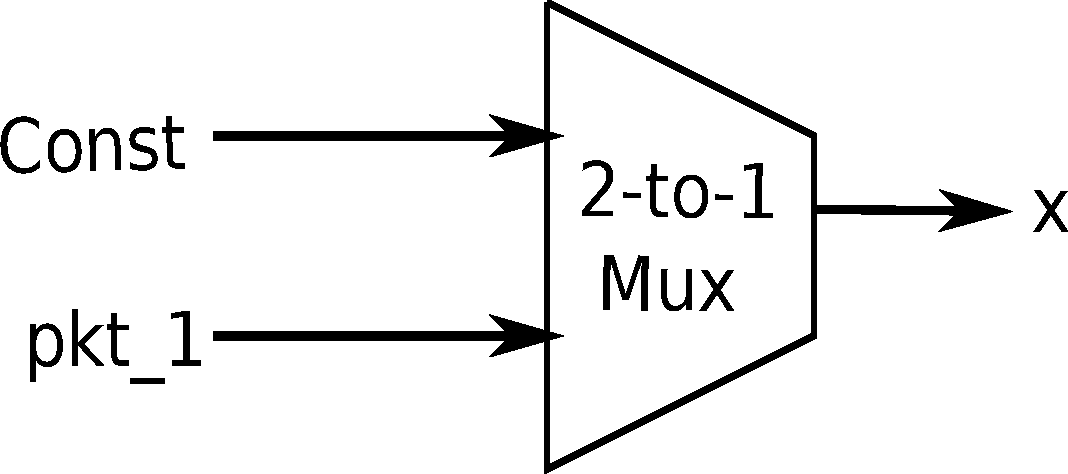
\includegraphics[width=0.2\textwidth]{rw.pdf} & 1 \\
  \hline
  ReadAddWrite (RAW) & 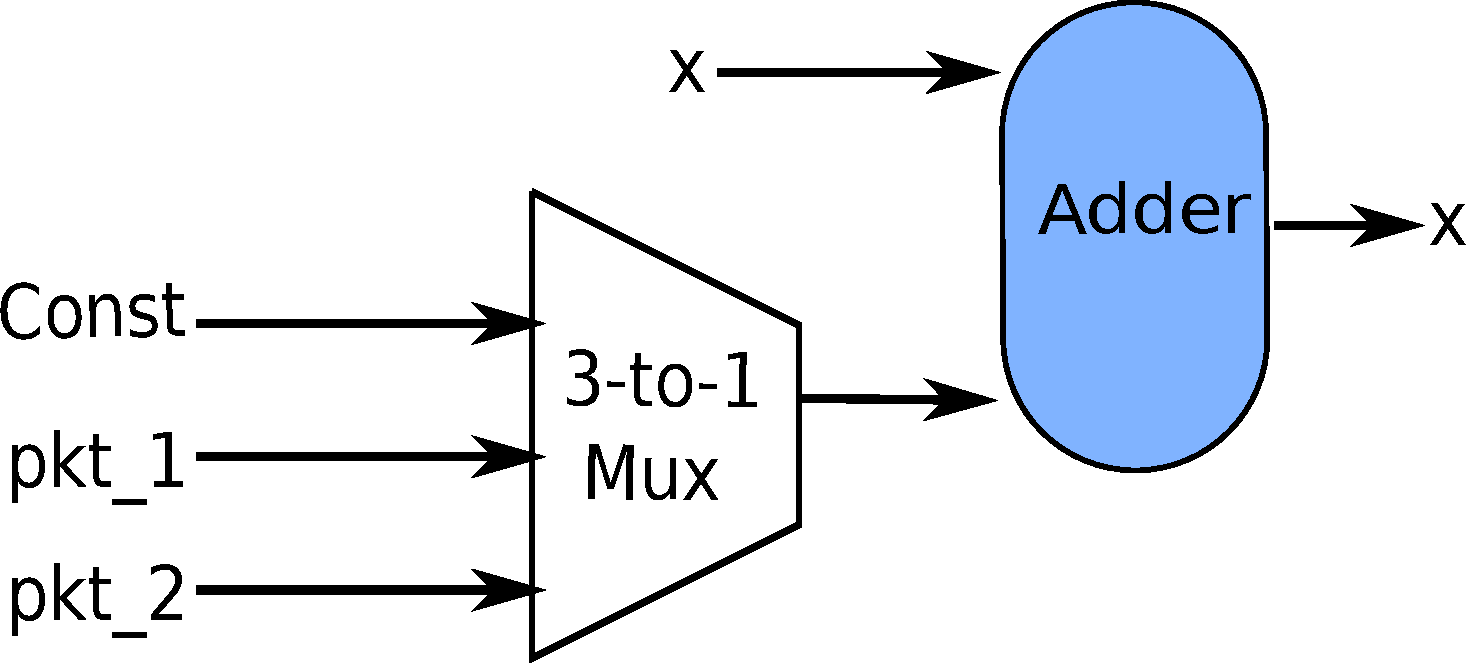
\includegraphics[width=0.2\textwidth]{raw.pdf} & 2\\
  \hline
  \pbox{0.1\textwidth}
  {Predicated\\
  ReadAddWrite (PRAW)} & 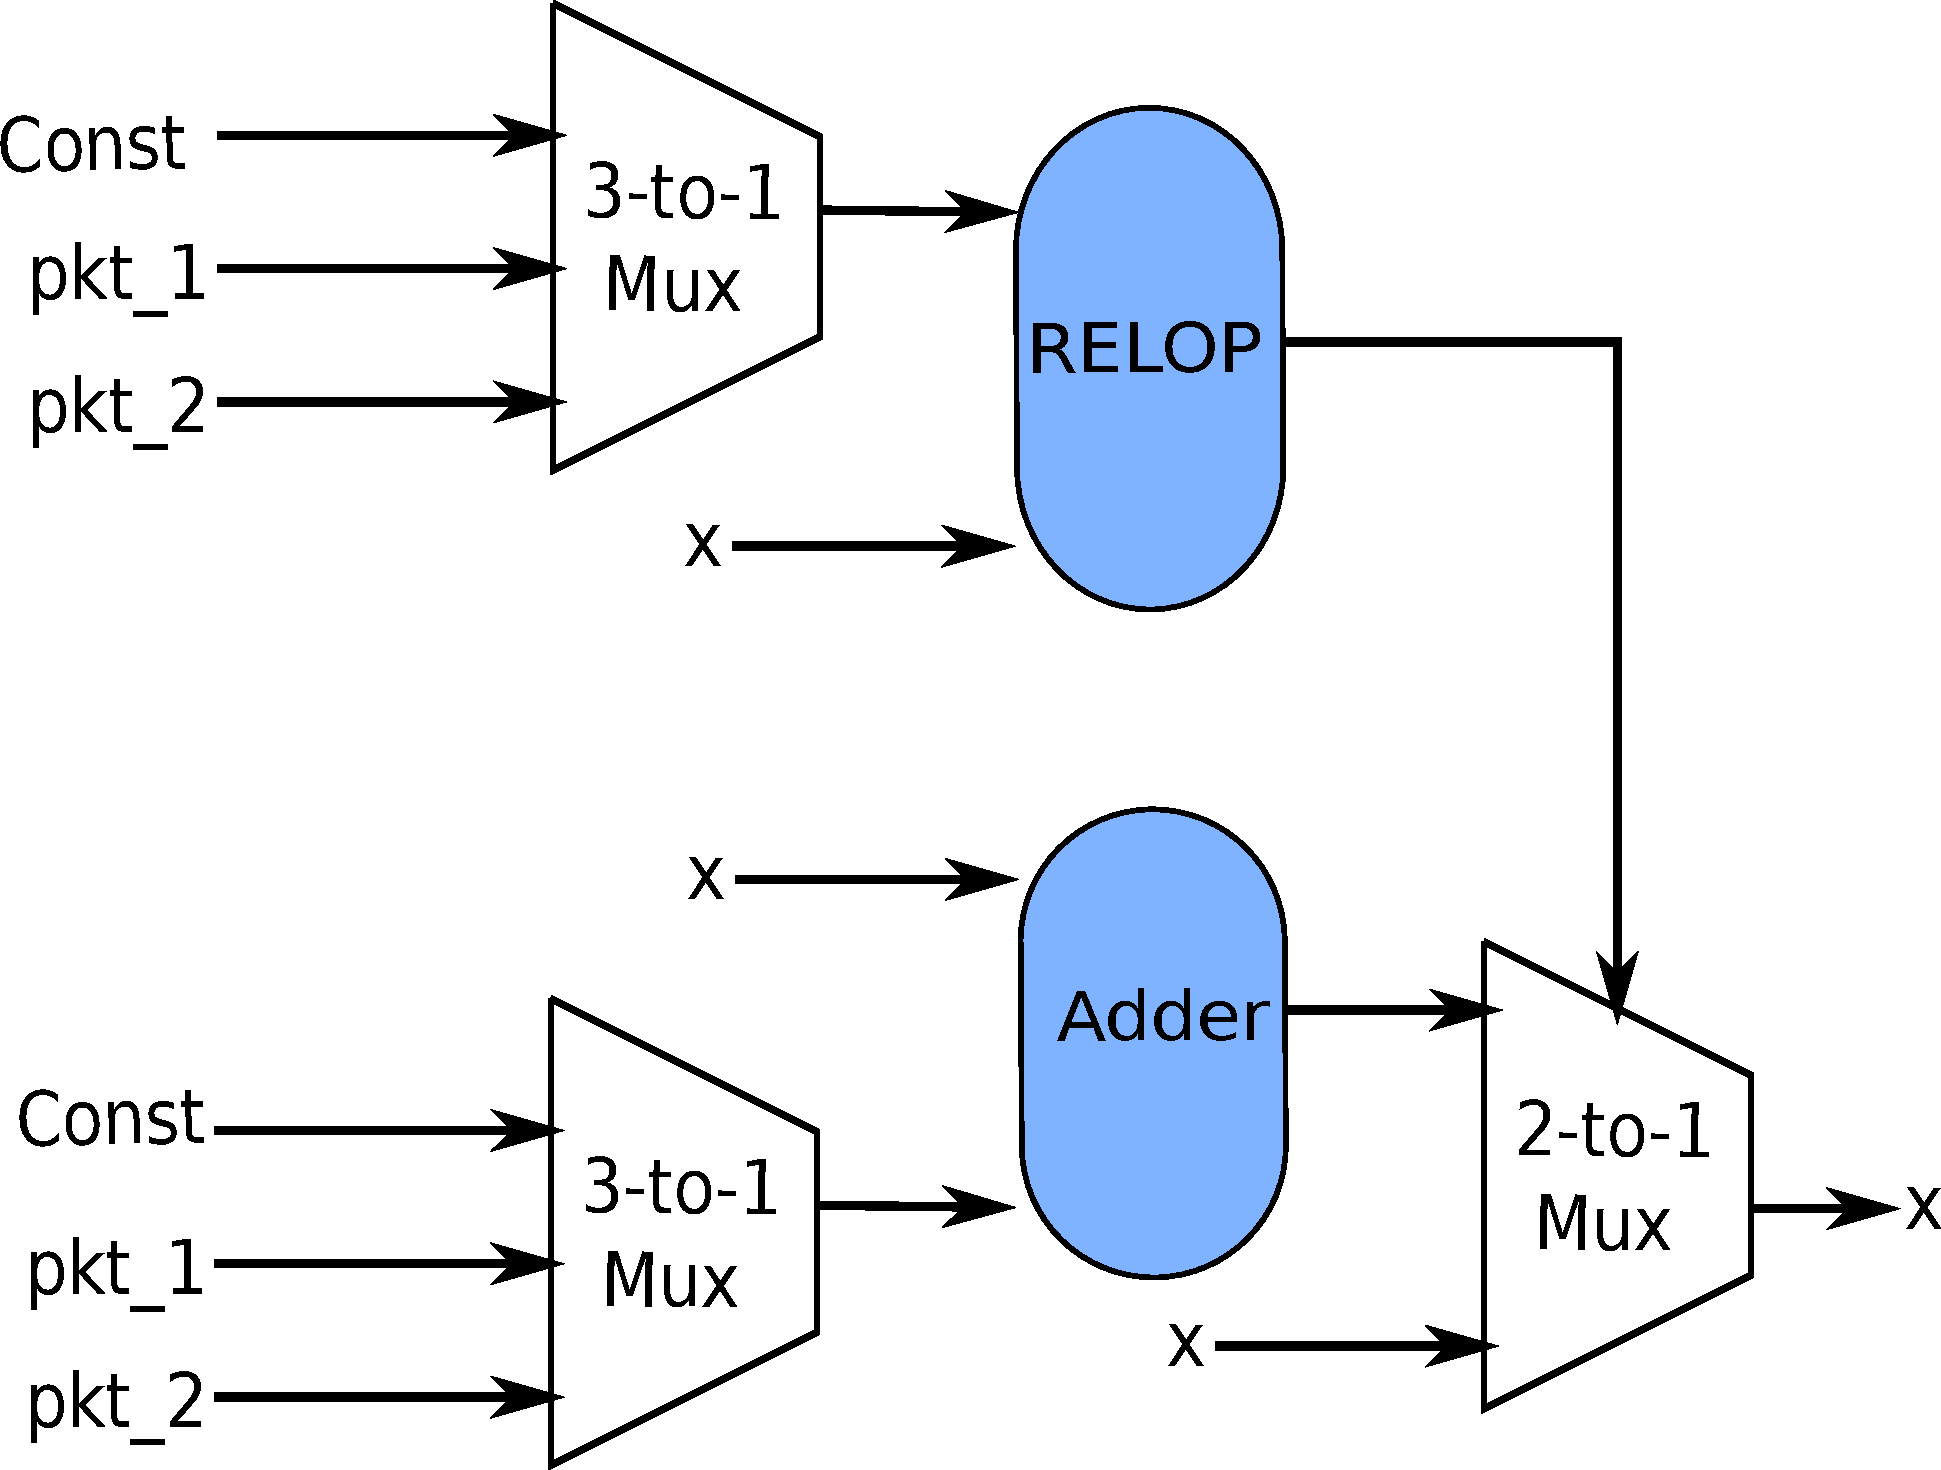
\includegraphics[width=0.3\textwidth]{pred_raw.pdf}  & 3\\
  \hline
  \end{tabular}
\end{scriptsize}
\caption{Circuit depth and propagation delay increases with complexity of atoms.}
  \label{fig:circuit_depth}
\end{table}

\begin{table*}[!t]
  \begin{tabular}{|p{0.16\textwidth}|p{0.47\textwidth}|p{0.09\textwidth}|p{0.06\textwidth}|p{0.07\textwidth}|}
\hline
Algorithm & Stateful computation & Least expressive atom & Pipeline depth, width & Ingress or Egress Pipeline?\\
\hline
\pbox{0.16\textwidth}{Bloom filter~\cite{bloom}\\(3 hash functions)} & \pbox{0.54\textwidth}{Set membership bit on every packet.} & Write & 4, 3 & Either \\
\hline
\pbox{0.16\textwidth}{Heavy Hitters~\cite{opensketch}\\(3 hash functions)} & Increment Count-Min Sketch~\cite{cormode} on every packet. & RAW & 10, 9 & Either \\
\hline
Flowlets~\cite{flowlets} & Update saved next hop if flowlet threshold is exceeded. & PRAW & 6, 2 & Ingress \\
\hline
RCP~\cite{rcp} & \pbox{0.47\textwidth}{Accumulate RTT sum if\\RTT is under maximum allowable RTT.} & PRAW & 3, 3 & Egress \\
\hline
\pbox{0.16\textwidth}{Sampled\\NetFlow~\cite{sampled_nflow}} & \pbox{0.47\textwidth}{Sample a packet if packet count reaches N;\\Reset count to 0 when it reaches N.} & IfElseRAW & 4, 2 & Either\\
\hline
HULL~\cite{hull} & Update counter for virtual queue. & Sub & 7, 1 & Egress \\
\hline
\pbox{0.16\textwidth}{Adaptive\\Virtual Queue~\cite{avq}} & Update virtual queue size and virtual capacity & Nested & 7, 3 & Ingress \\
\hline
CONGA~\cite{conga} & \pbox{0.54\textwidth}{Update best path's utilization/id if we see a better path.\\
                                           Update best path utilization alone if it changes.}  & Pairs & 4, 2 & Ingress\\
\hline
trTCM~\cite{trTCM} & Update token counts for each token bucket & Doesn't map & 7, 3 & Either \\
\hline
CoDel~\cite{codel} & \pbox{0.54\textwidth}{Update:\\Whether we are marking or not.\\Time for next mark.\\Number of marks so far.\\Time at which min. queuing delay will exceed target.}& Doesn't map & 15, 3 & Egress \\
\hline
\end{tabular}
\caption{Data-plane algorithms}
\label{tab:algos}
\end{table*}

To evaluate \pktlanguage, we express several data-plane algorithms
(Table~\ref{tab:algos}) using \pktlanguage and determine if they are
implementable on different \absmachine machines that provide different stateful
atoms (Table~\ref{tab:templates}). Appendix A contains circuit diagrams and
SKETCH code for these atoms.

We expressed most data-plane algorithms in \pktlanguage by simply translating
their imperative code/pseudocode to \pktlanguage. We did, however, modify
CoDel. Because CoDel drops from the head of a queue, it uses a
loop~\cite{codel_code} to repeatedly dequeue packets until it can send one out.
We replaced the loop with an if statement and mark packets instead of dropping
them. This reflects the reality that a switch running at line rate can dequeue
packets exactly once. Dropping these dequeued packets, instead of marking them,
leads to an idle line and wasted capacity.

\subsection{Experimental procedure}
As mentioned in \S\ref{ss:code_gen}, we consider only stateful atoms and assume
stateless codelets map one-to-one to stateless atoms for all \absmachine
machines. For simplicity, the stateful atoms only permit updates to state
variables and forbid packet field updates mixed in with these state updates.
Assuming the \absmachine machine provides an atom to read a state
variable\footnote{The inability to read a state variable renders it
powerless!}, such field updates can be treated as stateless operations in
subsequent pipeline stages.

We also assume every \absmachine machine provides exactly one kind of stateful
atom although we don't restrict the number of instances of this stateful atom.
Table~\ref{tab:templates} gradually increases the capability of this single
atom.  We designed the atoms in Table~\ref{tab:templates}, and hence the
\absmachine machines providing them, to form a containment hierarchy: each atom
can express all data-plane algorithms that its predecessor can.

We now consider every atom/\absmachine machine from Table~\ref{tab:templates},
and every data-plane algorithm from Table~\ref{tab:algos} to determine if the
algorithm is \textit{implementable} on a particular \absmachine machine. We say
an algorithm is implementable on a \absmachine machine, if every stateful
codelet within the data-plane algorithm can be mapped (\S\ref{ss:code_gen}) to
the stateful atom provided by the \absmachine machine. Because atoms are
arranged in a containment hierarchy, we list the \textit{least expressive} atom
that can be used to implement a data-plane algorithm in Table~\ref{tab:algos}.

\subsection{Interpreting the results}
Table~\ref{tab:algos} tells a network programmer the minimal atom required to
run a data-plane algorithm at line rate. For an ASIC engineer designing
programmable switches, the same table describes the algorithms that are
implementable on a \absmachine machine with a specific stateful atom. For
instance, a \absmachine machine with the Pairs atom can implement the first
eight algorithms, while a machine with a simpler RAW atom can implement only
the first two.

We also extract broader lessons for designing programmable switching chips.
First, atoms supporting stateful operations on a single state variable are
sufficient for several data-plane algorithms (Bloom Filters through AVQ in
Table~\ref{tab:algos}). However, there are algorithms that need the ability to
update a pair of state variables based on the previous value of the pair. One
example is CONGA, whose code we reproduce below:
\begin{verbatim}
  if (p.util < best_path_util[p.src]) {
    best_path_util[p.src] = p.util;
    best_path[p.src] = p.path_id;
  } else if (p.path_id == best_path[p.src]) {
    best_path_util[p.src] = p.util;
  }
\end{verbatim}
Here, \texttt{best\_path} (the ID of the best path for a particular
destination) is updated conditioned on \texttt{best\_path\_util} (the
utilization of the best path to that destination)\footnote{p.src is the address
  of the host originating this utilization message, and hence the
destintation for the host receiving it and executing the CONGA algorithm.} and
vice versa. There is no way to separate the two state variables into separate
stages and guarantee correctness.
%TODO: Mihai: Add figure of CONGA's SCC here maybe?

The Pairs atom, where the update to a state variable is conditioned on a
predicate of a pair of state variables, allows us to implement CONGA at line
rate.  However, it is still insufficient for some algorithms. Algorithms such
as CoDel~\cite{codel} and the two-rate three-color meter~\cite{trTCM}(trTCM)
can still not run at line rate---even if a Pairs atom is available.

On a positive note, however, the codelets in both trTCM and CoDel are still
restricted to a pair of state variables.  We haven't yet encountered a case
where a triplet of state variables all fall in the same strongly connected
component/codelet, requiring a three-way state update.  We leave the problem of
approximating CoDel/trTCM to fit within a particular atom or conversely,
designing more complex atoms to support them to future work.

While an expressive atom is better for mapping more data-plane algorithms, it
does have a cost. A larger and more expressive atom takes up more gate area
when synthesized to a digital circuit and results in longer propagation delays.
As an illustration, consider the circuits for the first three atoms from Table
~\ref{tab:templates} shown in Figure~\ref{fig:circuit_depth}. We use the number
of elements that a wire has to pass through between input and output (the
circuit depth) as a proxy for propagation delay. We see that the circuit depth
increases as we add complexity to atoms. At some point, the propagation delay
may be large enough that the resulting circuit may not meet timing to sustain a
particular line rate. We plan to synthesize these atoms to circuits in a
standard cell library to study this further.

These results will change as programmable switches evolve and network
programmers push chip boundaries with new algorithms.  The larger takeaway is
that we can now begin to quantify the programmability-performance tradeoff that
chip designers have so far intuitively understood. Using the \pktlanguage
compiler, we can rigorously\footnote{Modulo inefficiencies in the compiler
itself.} determine if a particular set of data-plane algorithms can run at a
given line rate, given the atoms supported by the \absmachine machine at that
line rate.

%TODO: This isn't written as strongly as we could write this.
% Not sure whether we want to have this at all.
\subsection{Compilation times}
The data-plane algorithms that we consider are all under 100 LOC. Hence, our
front-end compilation times are negligible; compilation times are dominated by
SKETCH trying to map codelets to atoms. However, we limit the bit-width of
SKETCH holes to 5 bits because the constants we see in our algorithms are
small.  This reduces the search space for SKETCH.  The worst-case occurs when a
large algorithm does not map to a large atom, because then SKETCH has to rule
out every possible configuration. Quantitatively, our worst-case compilation
time is 10 seconds when CoDel doesn't map to a \absmachine machine with the
Pairs atom.  This time will increase if we increase the bit width of constants
that SKETCH has to search; howerver, because the data-plane algorithms are
themselves small, we don't anticipate compilation times being a concern.

\section{Related work}
\label{s:related}
NPUs: Tradeoffs are different here. Each stage can do very very little on a switch relative to an NPU. NPUs are Turing-complete; here, on a switch, programs either fit or don't. If they don't fit, you need to approximate.

P4 compiler (Lavanya's work): Complementary backend.

CMU work on pipelining datapaths: Verilog and circuits.

P4 itself: Too low level. NetASM: Once P4 needs an IR, NetASM might be a good choice.

Click: P4 paper wrote it off. We think its worth revisiting here.

Fastpass or Flexplane: Say that you love the abstraction they propose,
but would love to do it at higher line rates.

Click, Maple, Flexplane: Proposed transactions first. We are inspired by them.

\section{Discussion}
\new{
Packet transactions provide a pathway to take algorithms that were hitherto
meant only for software routers and run them on emerging programmble line-rate
switching chips. However, more work must be done before packet transactions
are ready for production use.
}
\new{
\begin{CompactEnumerate}
\item With packet transactions, we strove for the strongest and simplest
semantics possible: transactional semantics that provide the notion of an
atomic and isolated block of code. Although these semantics make it easier to
reason about performance, they exclude algorithms that cannot be run exactly at
line rate. Are weaker semantics sensible? One possibility is approximating
transactional semantics by only processing a sampled packet stream.
This provides an increased time budget for each packet, potentially allowing
the packet to be {\em recirculated} through the pipeline multiple times
for packet processing. Another possibility is for the implementation to
be eventually consistent with the transactional model, perhaps by updating
state over many clock cycles and guaranteeing that it will be correct only if
there are no subsequent state updates.
\item Our current implementation doesn't handle multiple transactions and the
associated issues of composing transactions. A policy language to
specify multiple transactions executing on different, possibly overlapping,
subsets of packets is an area for future work.
%% \item Our compiler doesn't provide completeness: the guarantee that for any
%% algorithm, if there exists any way to map an algorithm to a line-rate switch,
%% it will be found. We haven't required this for the examples in our evaluation
%% because the compiler does find a solution if one exists. However, as we scale
%% to larger code examples, having this guarantee would be useful.
% This is confusing. The writing makes it sound like SKETCH is complete, but the compiler isn't.
% Removing for now.
\item Our compiler doesn't aggressively optimize. For instance, it may be
possible to fuse two stateful codelets that independently increment two
separate counters into the same instance of the Pairs atom. However, by
carrying out a one-to-one mapping from codelets to the atoms implementing them,
our compiler precludes these optimizations.  Developing an {\em optimizing}
compiler for packet transactions is an area for future work.
\item Finally, our design process for atoms is largely manual.  Formalizing
this design process and automating it into an atom-design tool would be useful
for switch designers. For instance, given a corpus of data-plane algorithms,
can we automatically mine this corpus for stateful and stateless codelets, and
design an atom (or atoms) that captures the computations required by some (or
all) of them?
%%\ac{would interleaving stmts from multiple transactions be a potential
%%optimization here (as in db transactions)?}
%% Possibly: I don't quite know how to reason about the semantics yet :) We should talk about this, sometime!
\end{CompactEnumerate}
}

\section{Conclusion}
\label{s:conclusion}

This paper presented \pktlanguage, a high-level language that allows
programmers to write packet-processing code using packet transactions:
sequential code blocks that run to completion on every packet before processing
the next one. The \pktlanguage compiler compiles packet transactions in
\pktlanguage to \absmachine, a family of abstract machines modeled after
emerging programmable line-rate switch architectures~\cite{flexpipe, xpliant,
rmt}. Our results suggest that it is possible to simultaneously have the
convenience of high-level programming and the performance of line-rate
switches, contrary to claims in~\cite{p4} that a high-level language is
insufficiently constrained for programming line-rate switches.

In light of those claims, our position is that---when carefully
constrained---it is possible to design a language that finds a sweet spot
between expressiveness and performance somewhere between the extremes of P4 as
it stands today and Click. P4 as a language is still evolving and we hope some
of these results prompt a larger conversation around the utility of having
higher-level abstractions, such as transactions, in P4. As this paper shows,
these abstractions come at no cost to performance. While much work remains
before packet transactions can run on real hardware, we hope to have convinced
the reader that it is possible.


\medskip
\noindent
\textbf{Acknowledgements.} We thank our shepherd, Bruce Maggs, the anonymous SIGCOMM reviewers, Amy
Ousterhout, and Pratiksha Thaker for their suggestions
that improved the presentation of the paper. This work was partly supported by
NSF grants CNS-1563826 and CNS-1563788. We thank the industrial partners of the
MIT Center for Wireless Networks and Mobile Computing (Wireless@MIT) for their
support.

%TODO: Need to make the figures larger everywhere.

\balance
{\small \bibliographystyle{abbrv}
\bibliography{paper}}

%% Atom, description, circuit, SKETCH
\newpage
\appendix
\section{SKETCH code and circuit diagrams for atoms}

\begin{table*}[!htbp]
\begin{scriptsize}
  \center
  \begin{tabular}{|p{0.09\textwidth}|p{0.73\textwidth}|p{0.04\textwidth}|}
      \hline
      Atom & Atom template & Element depth\\
\hline
\pbox{0.1\textwidth}{Write\\Figure~\ref{fig:rw}} &
{\begin{lstlisting}[style=customctable]
x = Mux2(pkt_1, Const());
\end{lstlisting}} &
1 \\

\hline
\pbox{0.1\textwidth}{ReadAddWrite\\(RAW)\\Figure~\ref{fig:raw}} &
{\begin{lstlisting}[style=customctable]
x = Opt(x) + Mux2(pkt_1, Const());
\end{lstlisting}} &
2 \\

\hline
\pbox{0.1\textwidth}
{Predicated\\
ReadAddWrite\\(PRAW)\\Figure~\ref{fig:praw}} &
{\begin{lstlisting}[style=customctable]
if (rel_op(Opt(x), Mux3(pkt_1, pkt_2, Const()))) {
  x = Opt(x) + Mux3(pkt_1, pkt_2, Const());
}
\end{lstlisting}} &
3 \\

\hline
\pbox{0.1\textwidth}
{If-Else\\
ReadAddWrite\\(IfElseRAW)\\Figure~\ref{fig:ifelseraw}} &
{\begin{lstlisting}[style=customctable]
if (rel_op(Opt(x), Mux3(pkt_1, pkt_2, Const()))) {
  x = Opt(x) + Mux3(pkt_1, pkt_2, Const());
} else {
  x = Opt(x) + Mux3(pkt_1, pkt_2, Const());
}
\end{lstlisting}} &
3 \\

\hline
\pbox{0.1\textwidth}
{Subtract (Sub)\\Figure~\ref{fig:sub}} &
{\begin{lstlisting}[style=customctable]
if (rel_op(Opt(x), Mux3(pkt_1, pkt_2, Const()))) {
  x = Opt(x) + Mux3(pkt_1, pkt_2, Const()) - Mux3(pkt_1, pkt_2, Const());
} else {
  x = Opt(x) + Mux3(pkt_1, pkt_2, Const()) - Mux3(pkt_1, pkt_2, Const());
}
\end{lstlisting}}&
4 \\

\hline
\pbox{0.1\textwidth}
{Nested Ifs\\(Nested)\\Figure~\ref{fig:nested}} &
{\begin{lstlisting}[style=customctable]
if (rel_op(Opt(x) + Mux2(pkt_1, pkt_2) - Mux2(pkt_1, pkt_2), Const())) {
 if (rel_op(Opt(x) + Mux2(pkt_1, pkt_2) - Mux2(pkt_1, pkt_2), Const())) {
  x = Opt(x) + Mux3(pkt_1, pkt_2, Const()) - Mux3(pkt_1, pkt_2, Const());
 } else {
  x = Opt(x) + Mux3(pkt_1, pkt_2, Const()) - Mux3(pkt_1, pkt_2, Const());
 }
} else {
 if (rel_op(Opt(x) + Mux2(pkt_1, pkt_2) - Mux2(pkt_1, pkt_2), Const())) {
  x = Opt(x) + Mux3(pkt_1, pkt_2, Const()) - Mux3(pkt_1, pkt_2, Const());
 } else {
  x = Opt(x) + Mux3(pkt_1, pkt_2, Const()) - Mux3(pkt_1, pkt_2, Const());
 }
}
\end{lstlisting}} &
6 \\

\hline
\pbox{0.1\textwidth}
{Paired Updates\\(Pairs)\\Figure~\ref{fig:pairs}} &
{\begin{lstlisting}[style=customctable]
if (rel_op(Mux2(x, y) + Mux2(pkt_1, pkt_2) - Mux2(pkt_1, pkt_2), Const())) {
 if (rel_op(Mux2(x, y) + Mux2(pkt_1, pkt_2) - Mux2(pkt_1, pkt_2), Const())) {
  x = Opt(x) + Mux3(pkt_1, pkt_2, Const()) - Mux3(pkt_1, pkt_2, Const());
  y = Opt(y) + Mux3(pkt_1, pkt_2, Const()) - Mux3(pkt_1, pkt_2, Const());
 } else {
  x = Opt(x) + Mux3(pkt_1, pkt_2, Const()) - Mux3(pkt_1, pkt_2, Const());
  y = Opt(y) + Mux3(pkt_1, pkt_2, Const()) - Mux3(pkt_1, pkt_2, Const());
 }
} else if (rel_op(Mux2(x, y) + Mux2(pkt_1, pkt_2) - Mux2(pkt_1, pkt_2), Const())) {
 if (rel_op(Mux2(x, y) + Mux2(pkt_1, pkt_2) - Mux2(pkt_1, pkt_2), Const())) {
  x = Opt(x) + Mux3(pkt_1, pkt_2, Const()) - Mux3(pkt_1, pkt_2, Const());
  y = Opt(y) + Mux3(pkt_1, pkt_2, Const()) - Mux3(pkt_1, pkt_2, Const());
 } else {
  x = Opt(x) + Mux3(pkt_1, pkt_2, Const()) - Mux3(pkt_1, pkt_2, Const());
  y = Opt(y) + Mux3(pkt_1, pkt_2, Const()) - Mux3(pkt_1, pkt_2, Const());
 }
}
\end{lstlisting}} &
6 \\
\hline

  \end{tabular}
  \end{scriptsize}
  \caption{SKETCH code for atoms described in Table~\ref{tab:templates}}
  \label{tab:atom_code}
\end{table*}

\FloatBarrier
The appendix provides circuit diagrams and SKETCH code for the atoms in
Table~\ref{tab:templates}. Table~\ref{tab:sketch_constructs} summarizes the
SKETCH notation we use in this section.
\begin{table}[!htbp]
  \begin{scriptsize}
  \begin{tabular}{p{0.3\columnwidth}p{0.7\columnwidth}}
  SKETCH construct & Description \\
  \hline
  MuxN(a1, a2, \dots, aN) & \pbox{0.7\columnwidth}{N-to-1 multiplexer with enable bit.\\If enabled, return one of a1, a2, \dots aN.\\If disabled, return 0.}\\
  Opt(a)        & Return a or 0. \\
  rel\_op(x, y) & Return one of $x < y$, $x > y$, $x != y$, $x == y$.\\
  Const() & Return an integer constant in the range [0, 31].\footnote{We restrict constants to 5 bits because all constants in our dataplane algorithms are under 32. Larger ranges increase synthesis time.} \\
  x, y & State variables \\
  pkt\_1, pkt\_2 & Packet fields \\
  \end{tabular}
  \end{scriptsize}
  \caption{SKETCH notation used in atom templates}
  \label{tab:sketch_constructs}
\end{table}

\FloatBarrier

\begin{figure}[!htbp]
  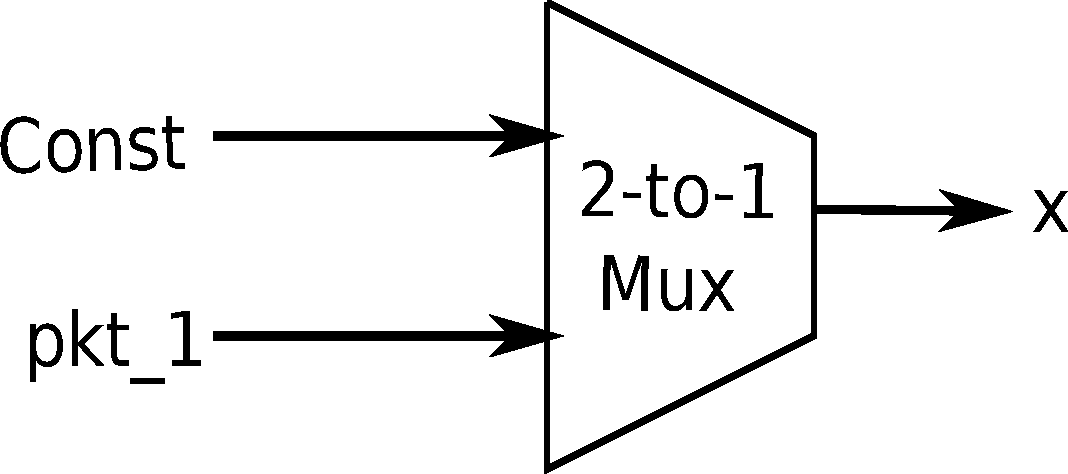
\includegraphics[width=\columnwidth]{rw.pdf}
  \caption{Circuit for Write atom with depth 1.}
  \label{fig:rw}
\end{figure}

\FloatBarrier

\begin{figure}[!htbp]
  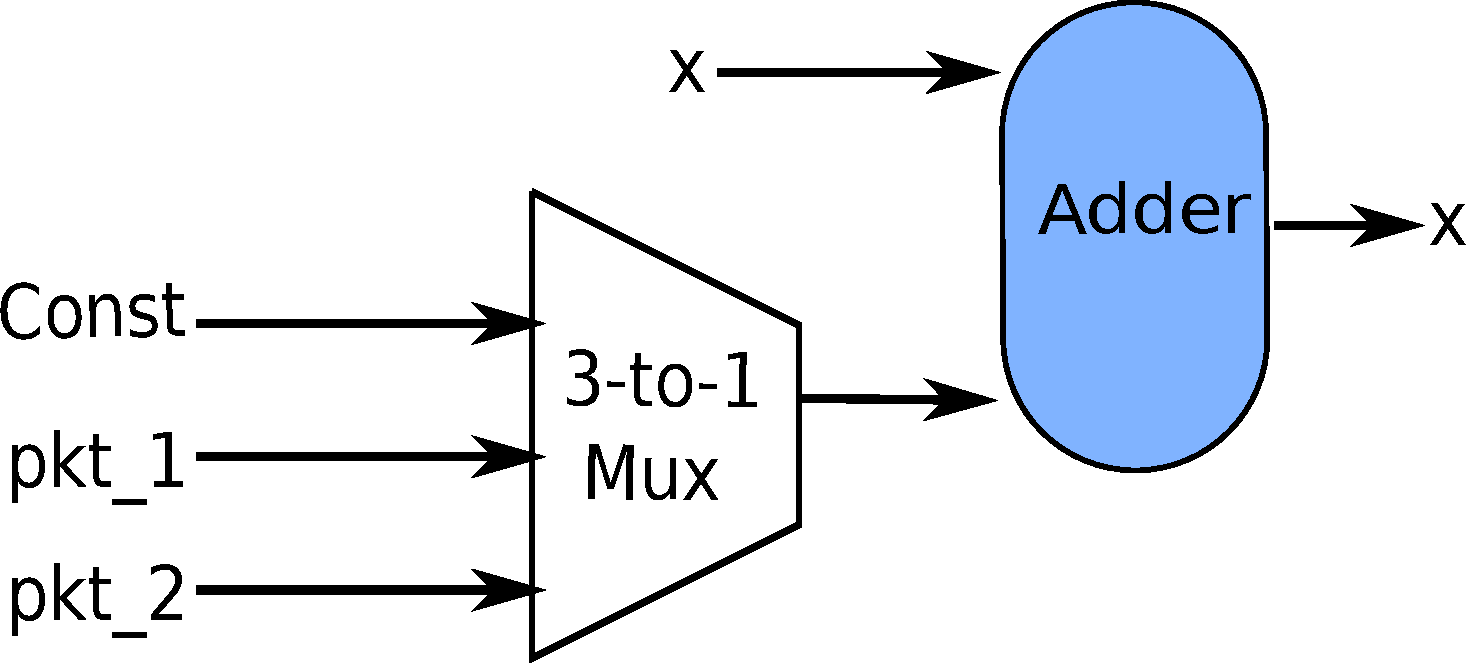
\includegraphics[width=\columnwidth]{raw.pdf}
  \caption{Circuit for RAW atom with depth 2.}
  \label{fig:raw}
\end{figure}

\FloatBarrier

\begin{figure}[!htbp]
  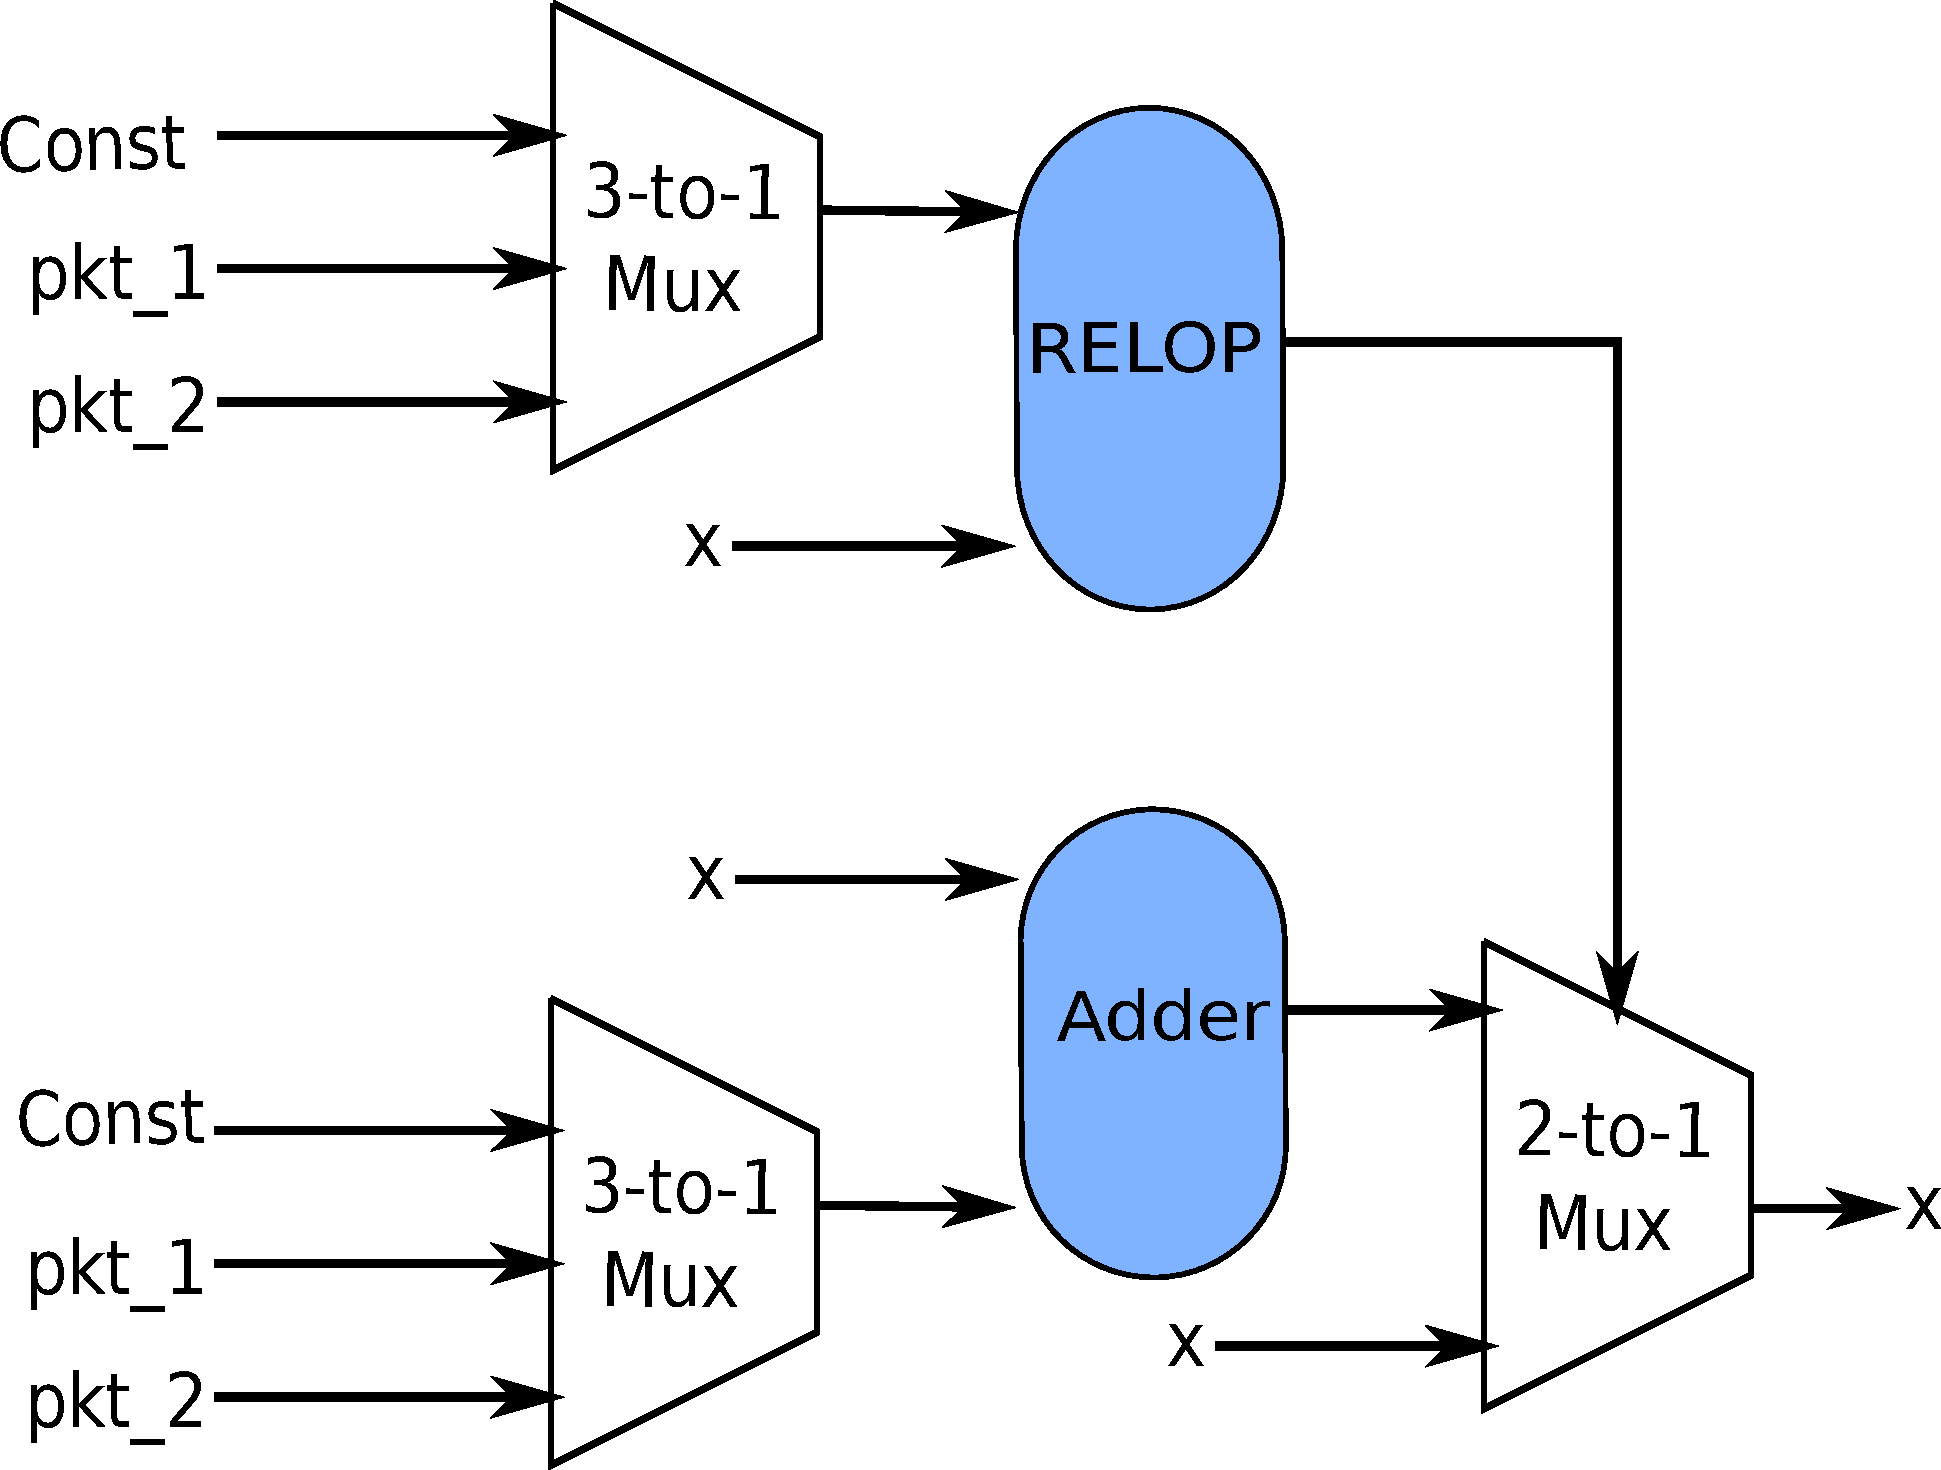
\includegraphics[width=\columnwidth]{pred_raw.pdf}
  \caption{Circuit for PRAW atom with depth 3.}
  \label{fig:praw}
\end{figure}

\FloatBarrier

\begin{figure}[!htbp]
  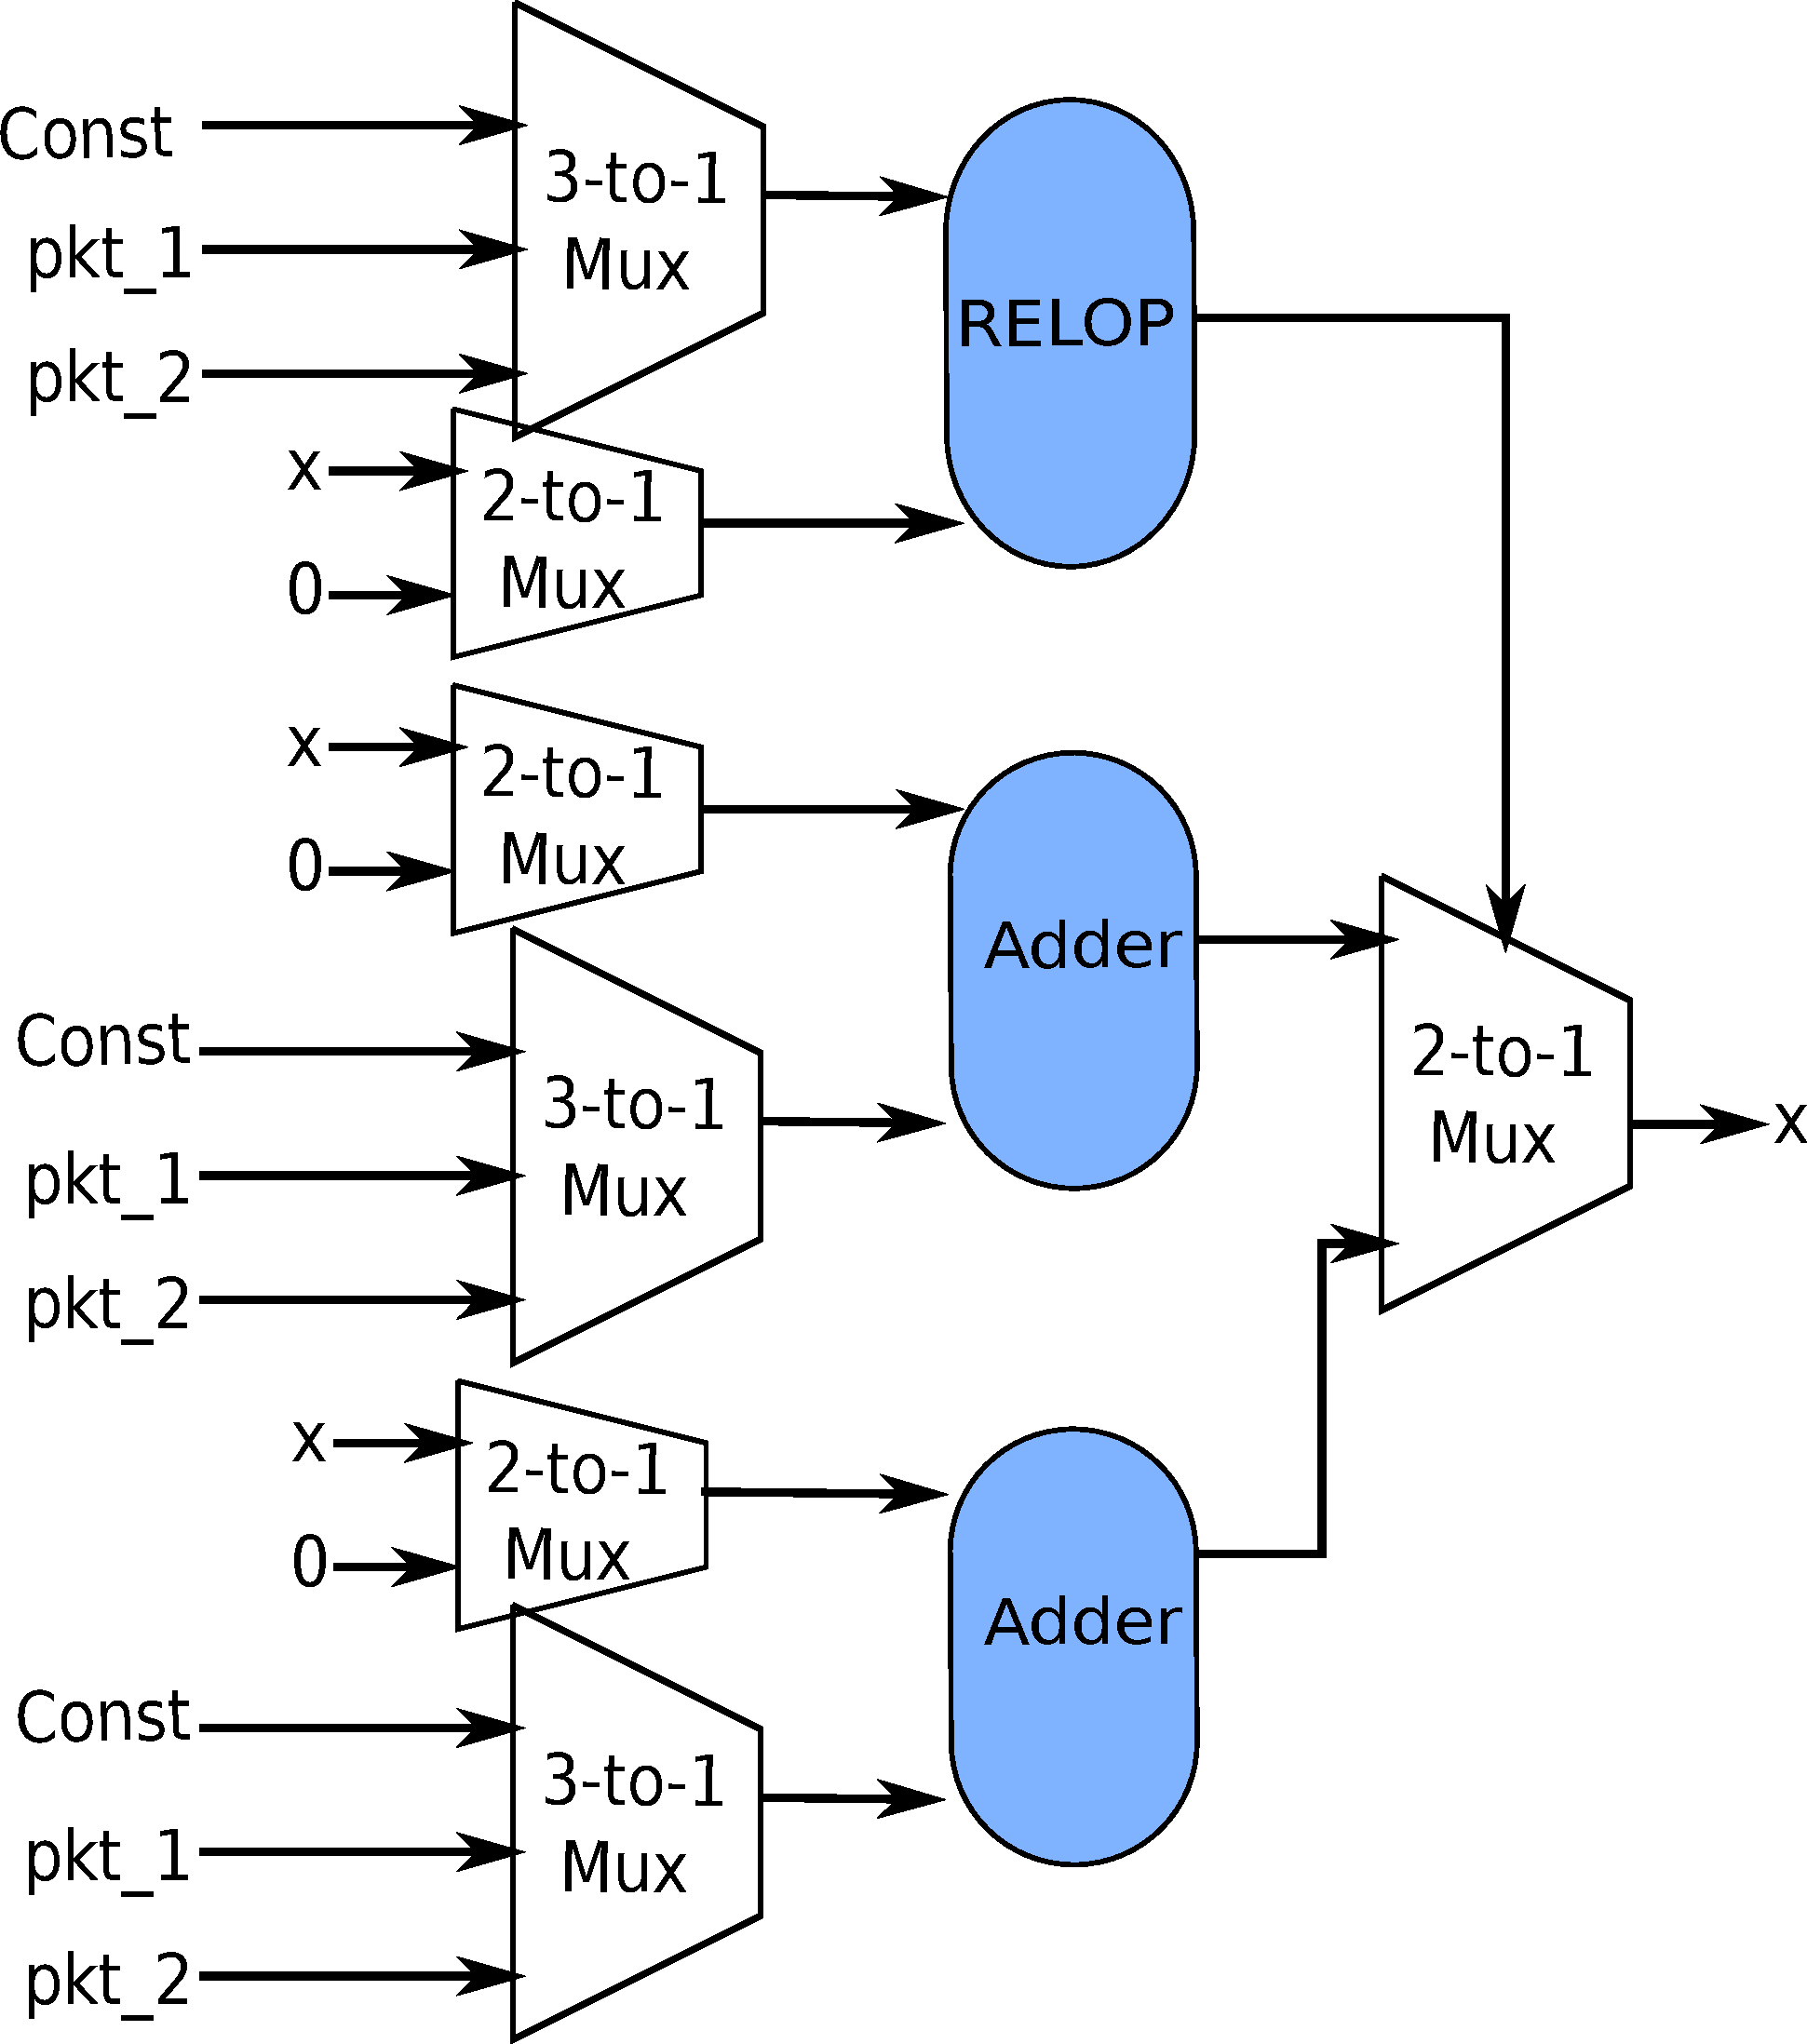
\includegraphics[width=\columnwidth]{if_else.pdf}
  \caption{Circuit for IfElseRAW atom with depth 3.}
  \label{fig:ifelseraw}
\end{figure}

\FloatBarrier

\begin{figure}[!htbp]
  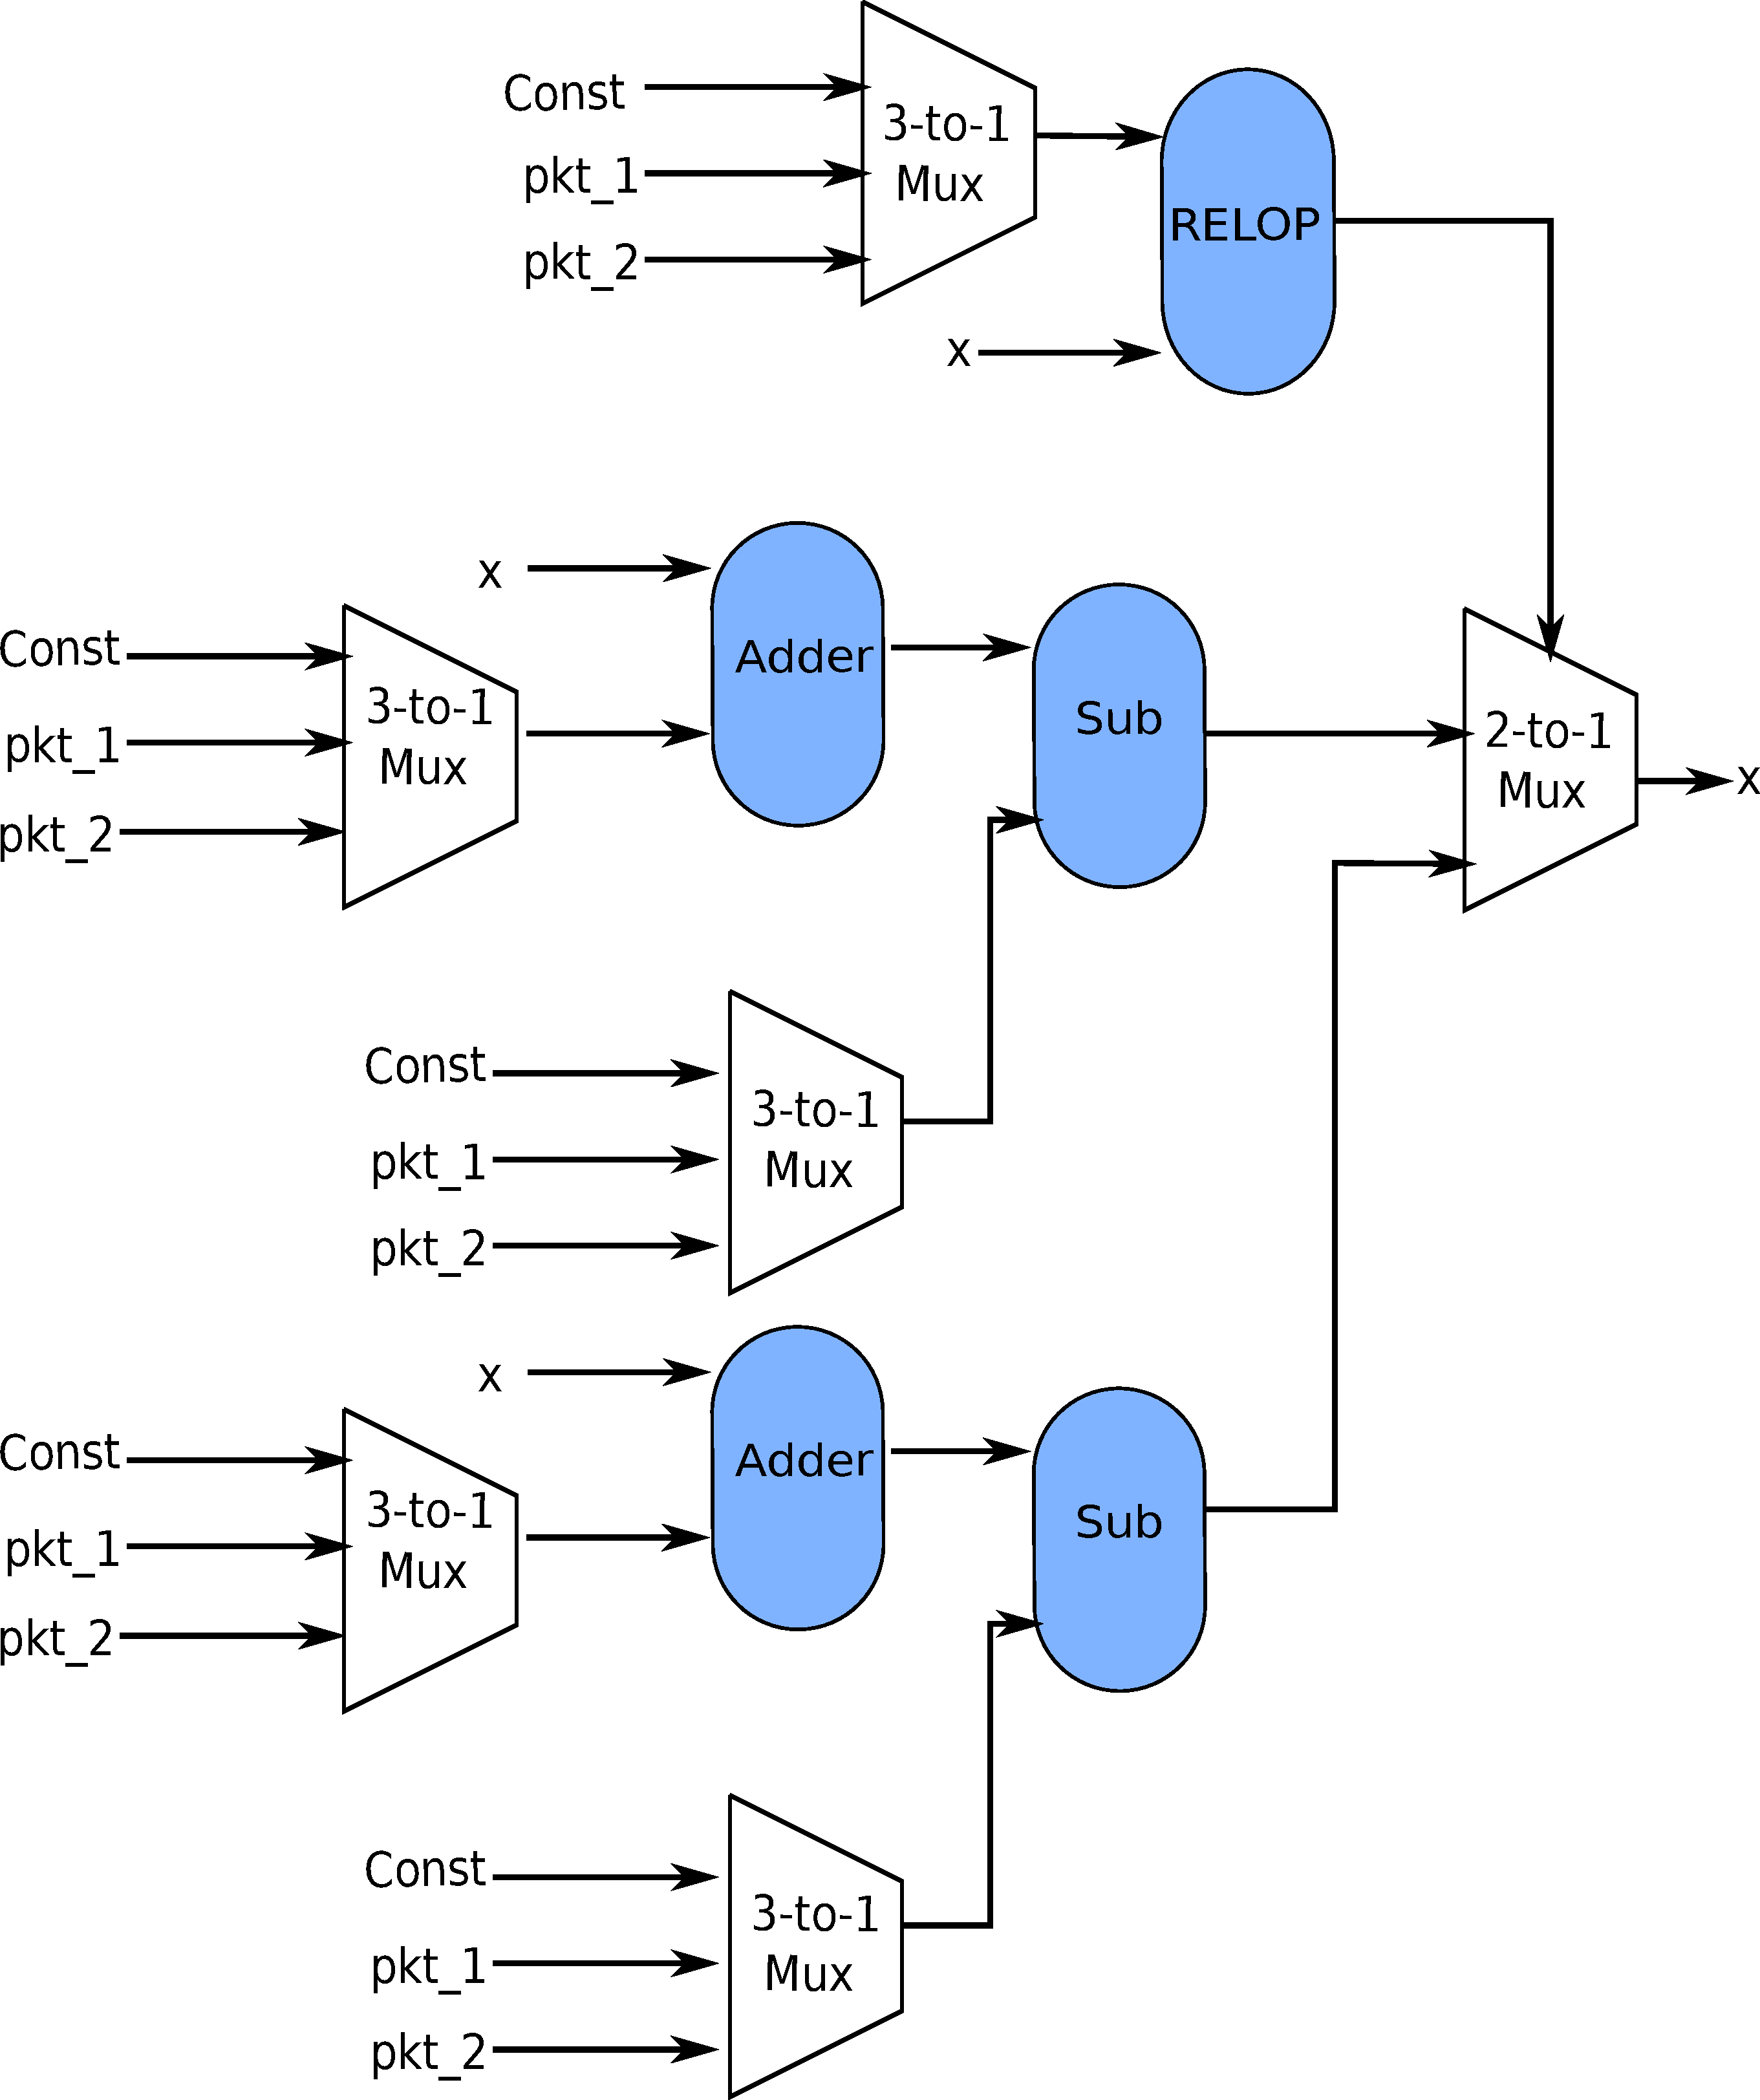
\includegraphics[width=\columnwidth]{sub.pdf}
  \caption{Circuit for Sub atom with depth 4.}
  \label{fig:sub}
\end{figure}

\FloatBarrier

\newpage
\begin{figure*}[!htbp]
  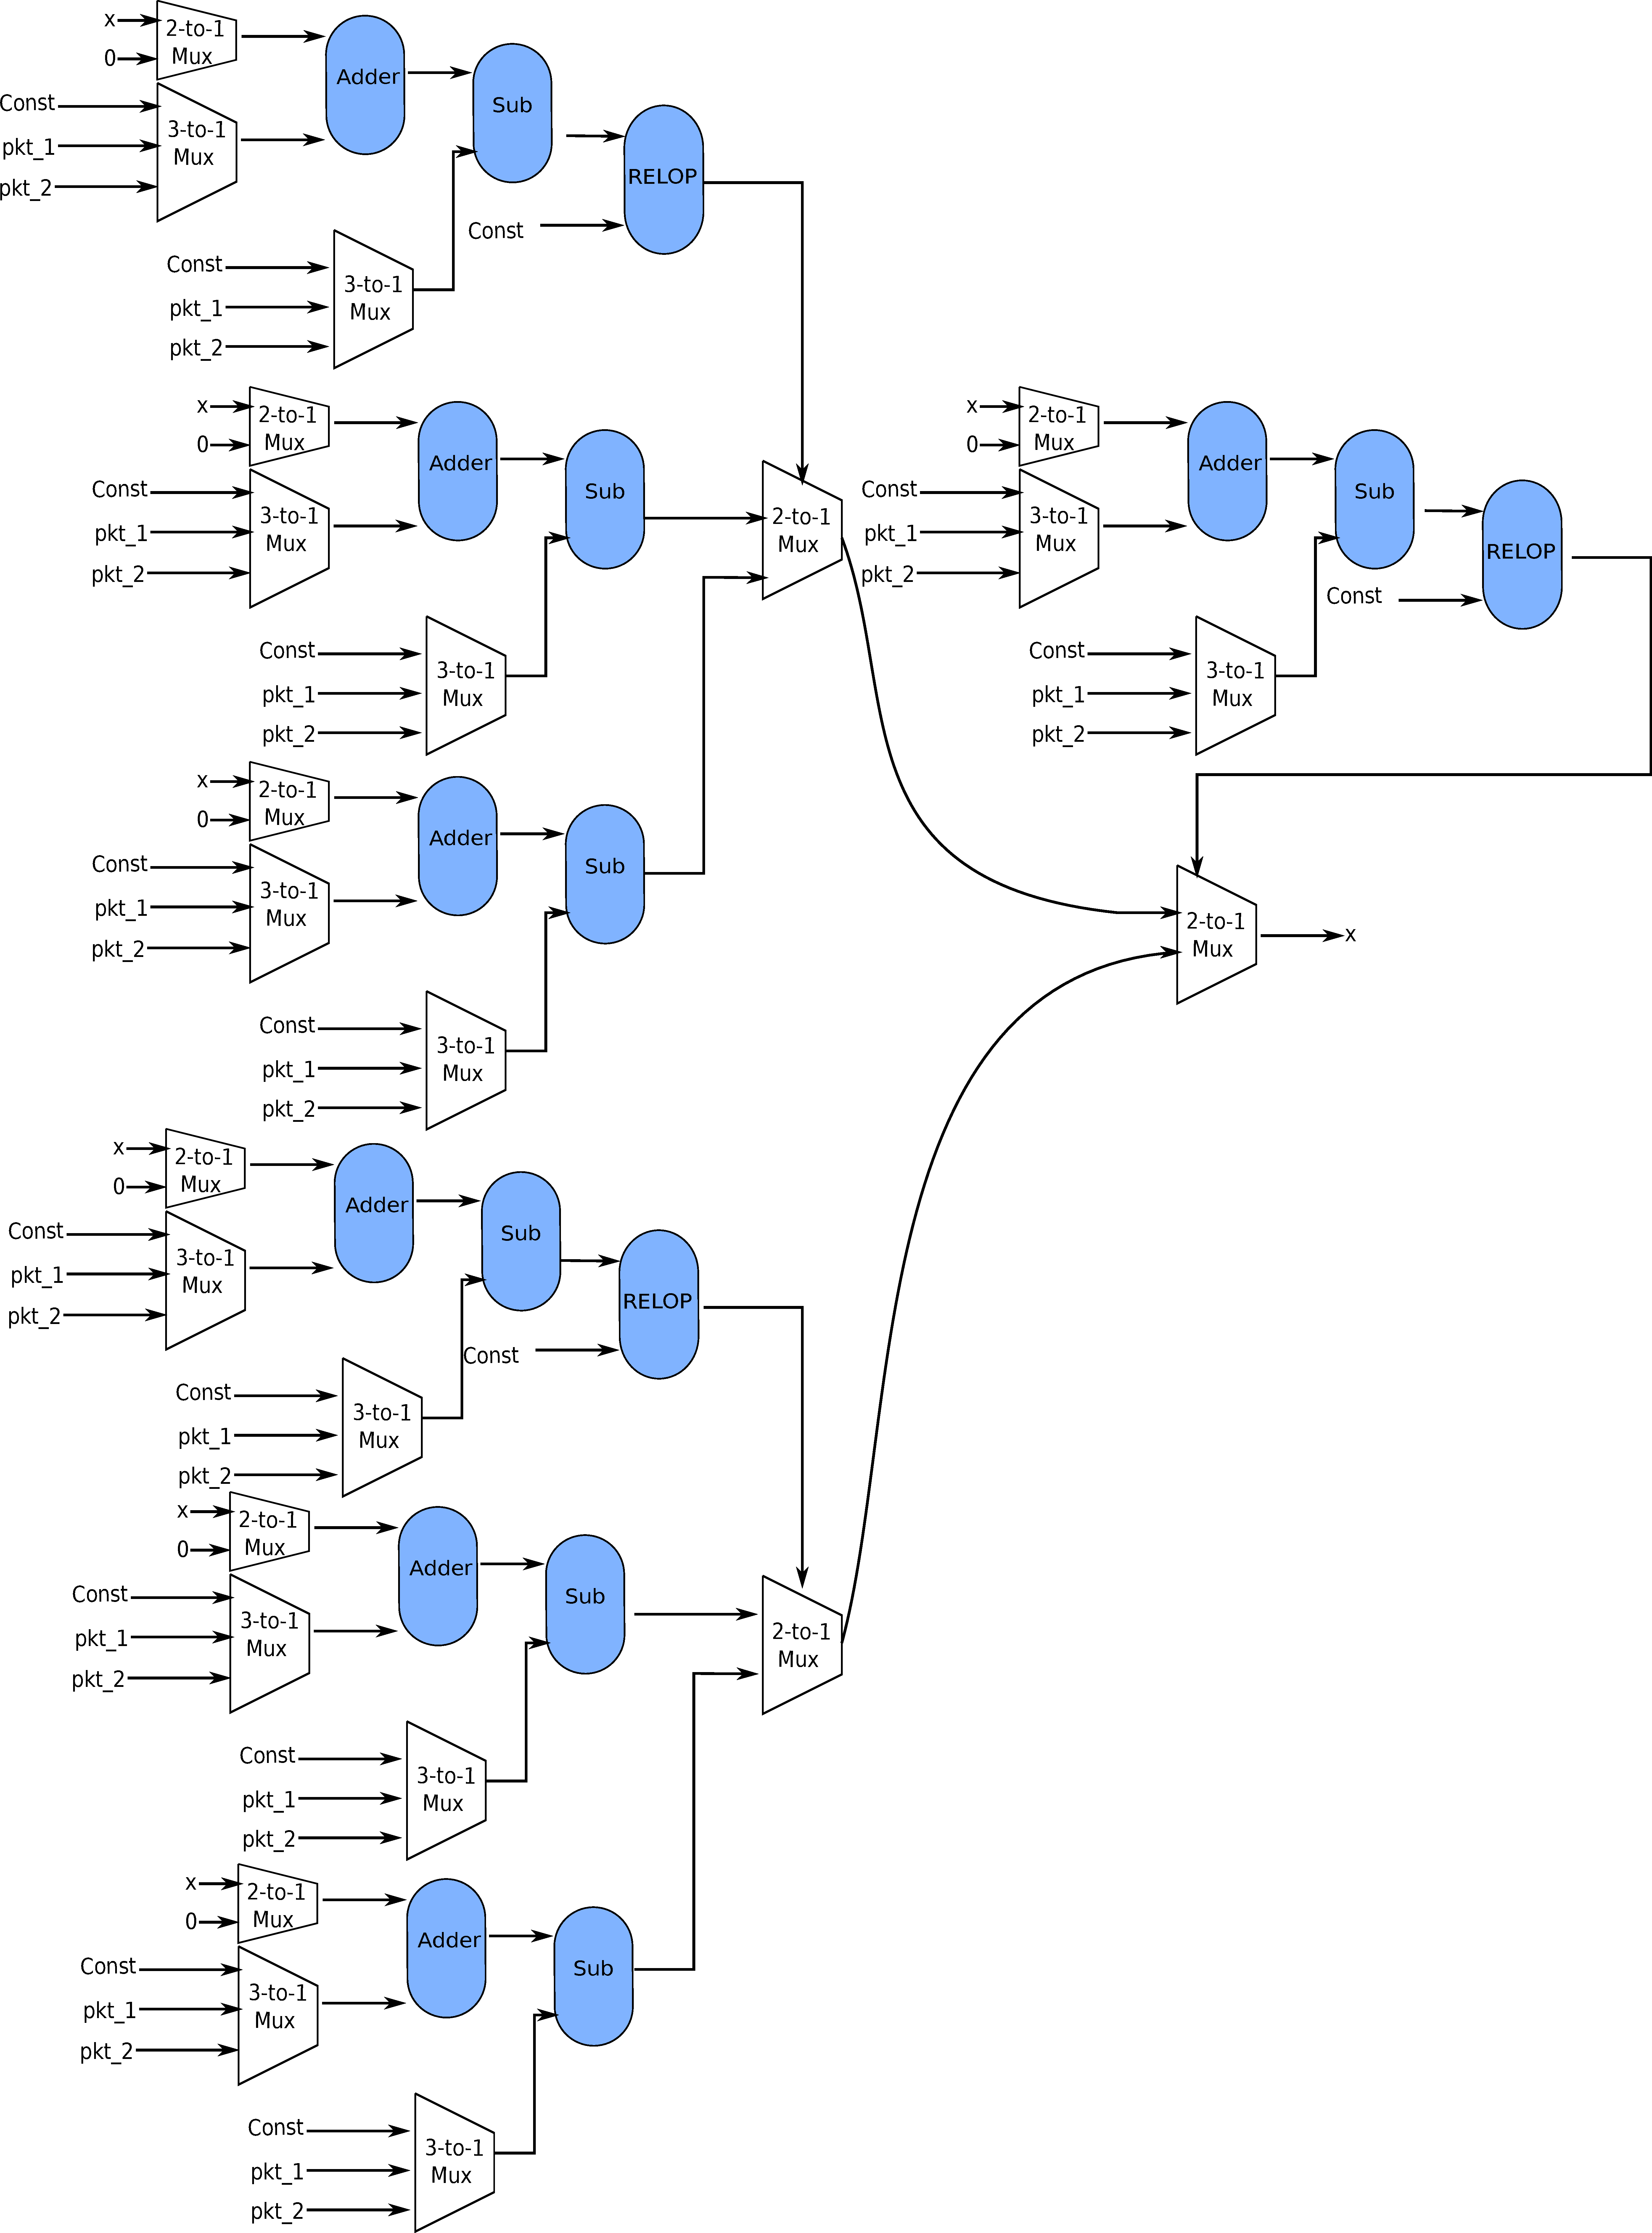
\includegraphics[width=\textwidth]{nested.pdf}
  \caption{Circuit for Nested atom with depth 6.}
  \label{fig:sub}
\end{figure*}

\FloatBarrier

\newpage
\begin{figure*}[!htbp]
  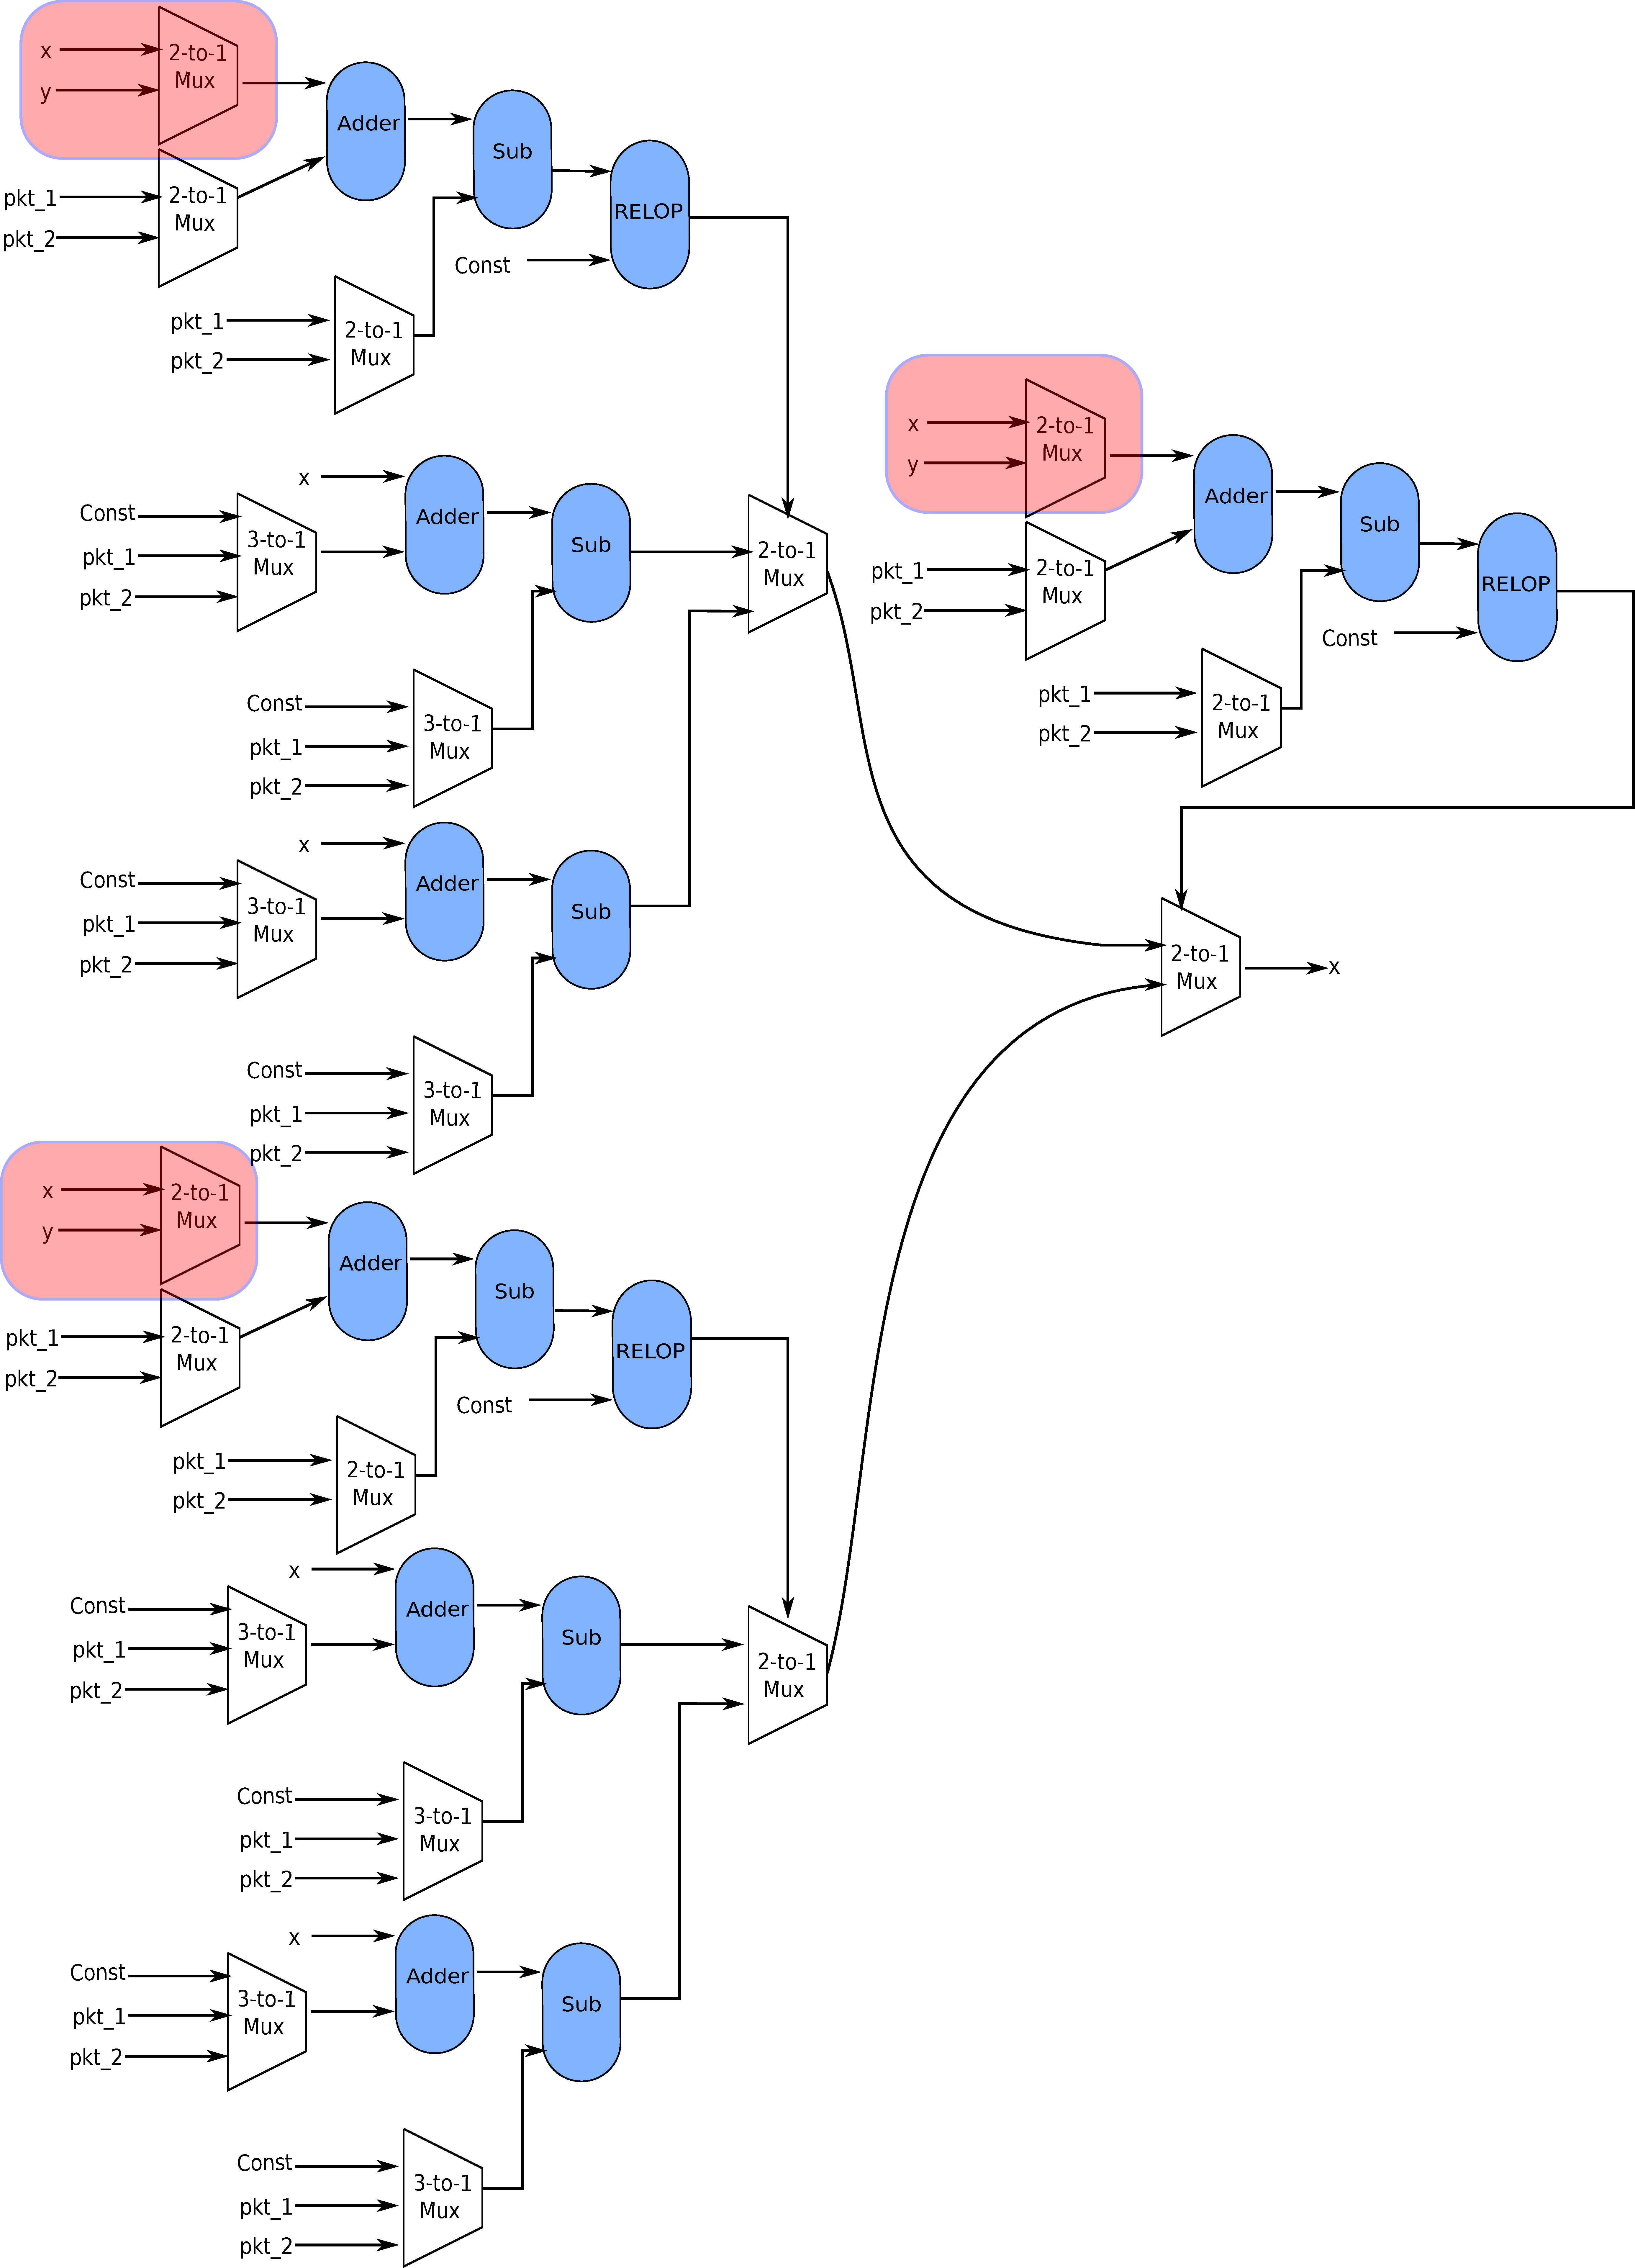
\includegraphics[width=\textwidth]{pairs.pdf}
  \caption{One-half of the circuit for the Pairs atom with depth 6. The other
  half is identical, except that it updates y instead of x, and isn't shown for
simplicity. The shaded regions denote the differences in the Pairs atom
relative to the Nested atom: the predicates can depend on both x and y in the Pairs
atom.}
  \label{fig:sub}
\end{figure*}

\end{document}
